\thispagestyle{toancuabinone}
\pagestyle{toancuabi}
\everymath{\color{toancuabi}}
%\blfootnote{$^1$\color{toancuabi}Đại học Thăng Long.}
\graphicspath{{../toancuabi/pic/}}
\begingroup
\AddToShipoutPicture*{\put(0,616){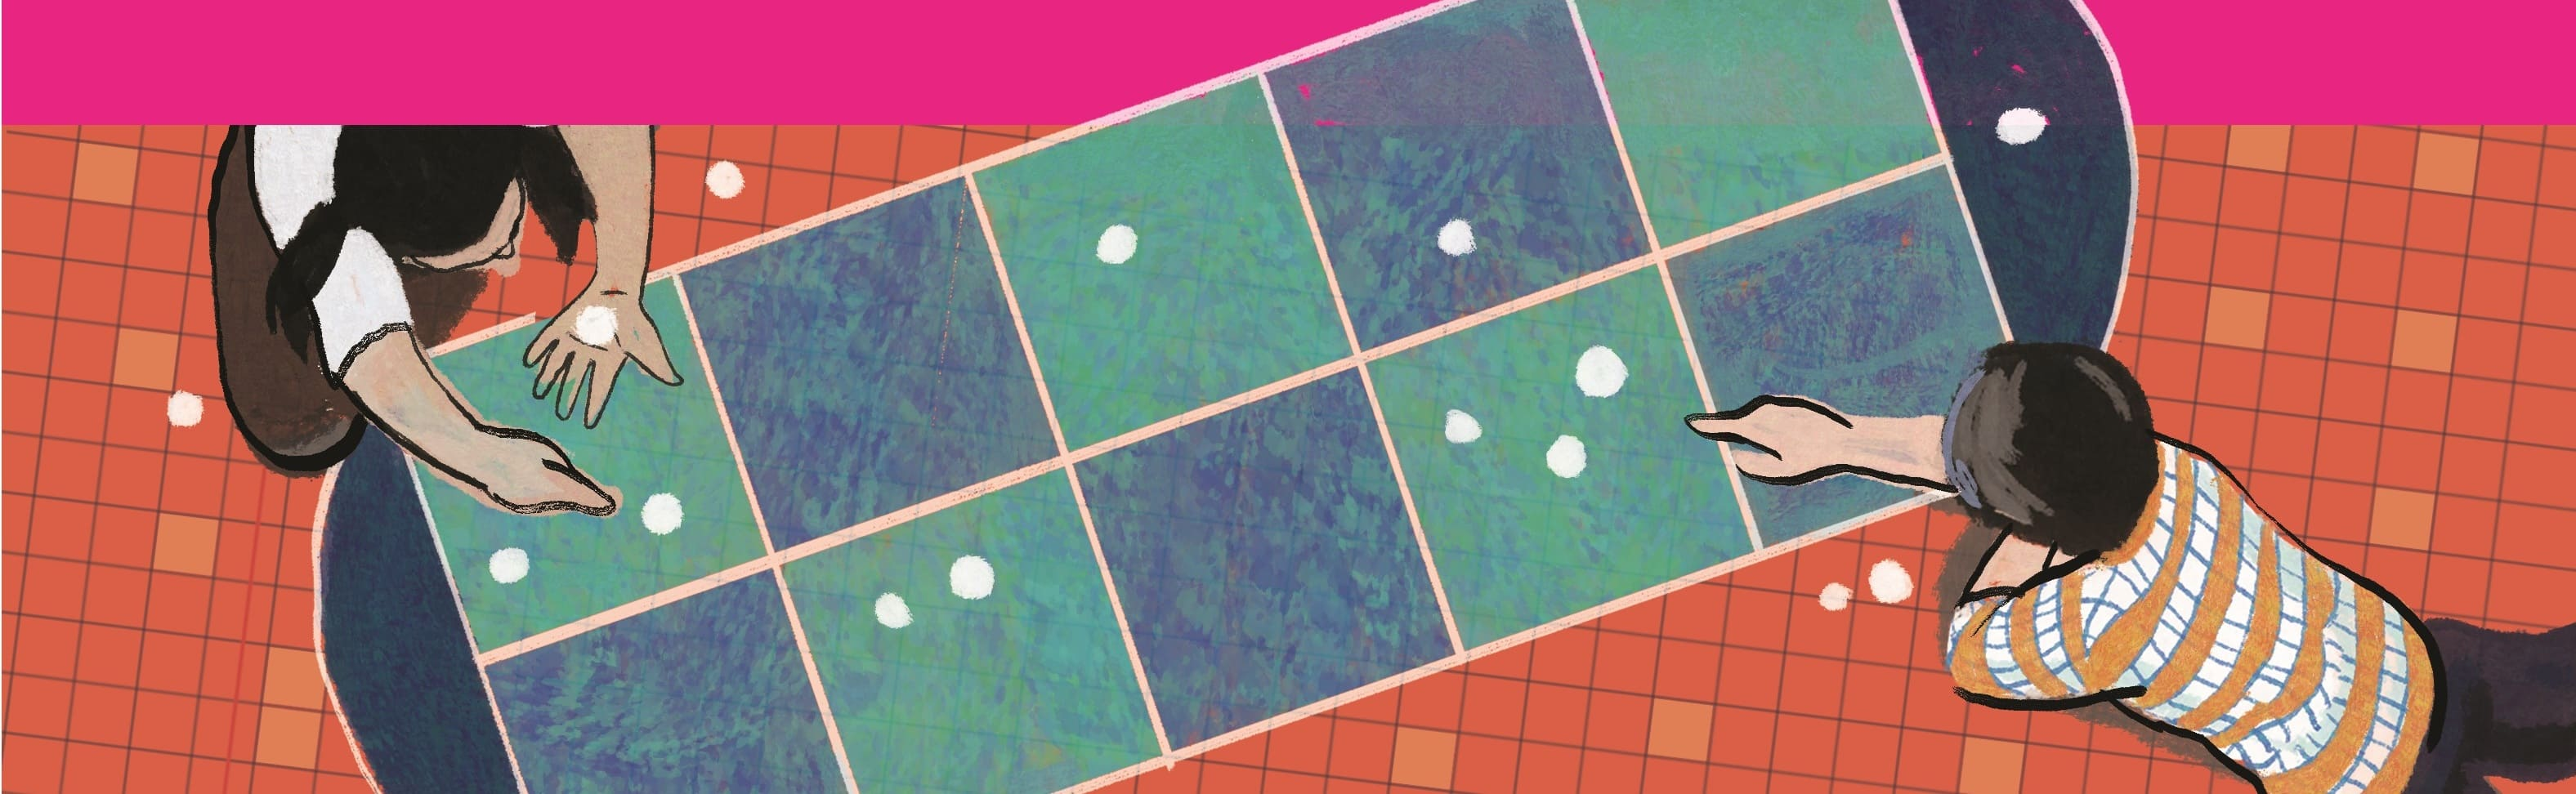
\includegraphics[width=19.3cm]{../bannertoancuabi}}}  
\AddToShipoutPicture*{\put(177,552){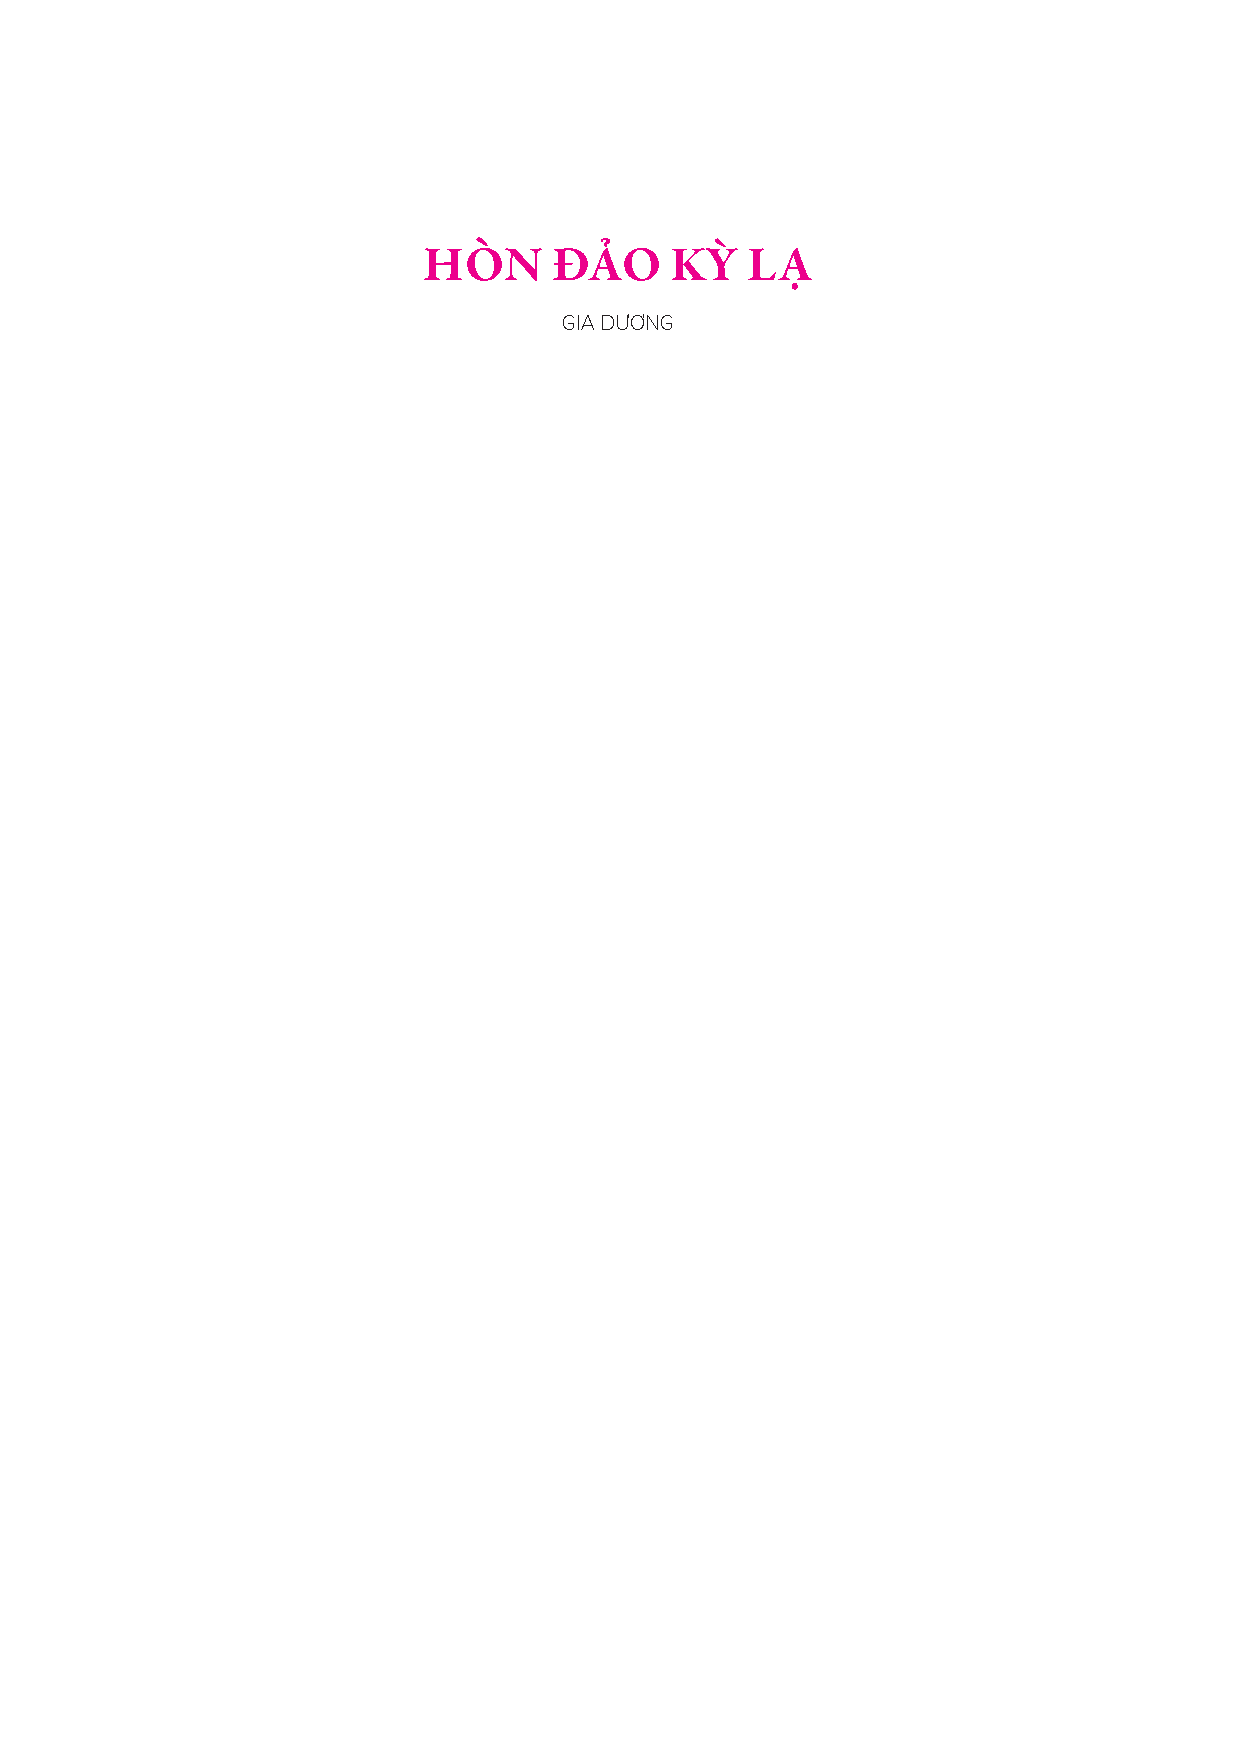
\includegraphics[scale=1]{../tieude.pdf}}} 
\centering
\endgroup

\vspace*{155pt}

\begin{multicols}{2}
	Thám tử Xuân Phong trong một lần đi du lịch cùng thanh tra Lê Kính tới một hòn đảo xa xôi tận bên Phi Châu được đặt chân tới một ngôi làng đẹp tuyệt diệu ẩn sau những cành cọ, rặng dừa xum xuê chạy dài bờ biển xanh ngắt trong veo. Trưởng làng đon đả mời hai người tới ngôi nhà lớn của cả làng để dự một lễ hội đặc biệt của người dân. Theo như chỉ dẫn từ công ty lữ hành, những người thổ dân ở làng đó chia thành hai họ tộc, họ Tutu chuyên nói thật và họ Titi lại chuyên nói dối. Khi bước vào căn nhà lớn, Xuân Phong đã thấy có $50$ người dân đảo ăn mặc\hspace*{123pt}\linebreak[6]những bộ quần\hspace*{123pt}\linebreak[6]áo màu sắc lộng\hspace*{123pt}\linebreak[6]lẫy dành riêng\hspace*{123pt}\linebreak[6]cho lễ hội và\hspace*{123pt}\linebreak[6]ngồi xung quanh\hspace*{123pt}\linebreak[6]một chiếc bàn\hspace*{123pt}\linebreak[6]tròn thật to đặt\hspace*{123pt}\linebreak[6]giữa phòng. Theo\hspace*{123pt}\linebreak[6]như tục lệ, $50$\hspace*{123pt}\linebreak[6]người sẽ lần lượt\hspace*{123pt}\linebreak[6]đứng lên và nếu\hspace*{123pt}\linebreak[6]số tuổi của hai\hspace*{123pt}\linebreak[6]người ngồi cạnh\hspace*{123pt}\linebreak[6]anh ta, tuổi\hspace*{123pt}\linebreak[6]người ngồi bên\hspace*{123pt}\linebreak[6]trái trước -- sau\hspace*{123pt}\linebreak[6]đó là người ngồi\hspace*{123pt}\linebreak[6]bên phải. Xuân\hspace*{123pt}\linebreak[6]Phong được biết trước trong sách hướng dẫn du lịch là: người tộc Tutu sẽ nói đúng cả hai con số này, còn người tộc Titi sẽ tăng một trong hai số tuổi của hai người ngồi cạnh (người nào theo cách anh ta tùy thích chọn) thêm $1$ tuổi còn giảm tuổi kia đi $1$ tuổi. Xuân Phong chỉ cần nghe xong và ghi chép lại $50$ câu nói  của $50$ người dân làng ngồi quanh bàn, sau một chút suy nghĩ, đã biết được ngay ai là người đến từ tộc nào, Tutu hay Titi. Làm sao mà thám tử lại tài thế nhỉ, các em có biết cách lập luận của Xuân Phong được hay không?
	
	\vspace*{280pt}
	\insertpic{159}{85}{0.54}{xp}
\end{multicols}
\newpage
\begingroup
\AddToShipoutPicture*{\put(112,672){
\includegraphics[scale=1]{../tieude11.pdf}}} 
\centering
\endgroup
\vspace*{35pt}

\begin{multicols}{2}
	$\pmb{1.}$ Bạn Tùng làm một số bài trắc nghiệm và sau đó sẽ lấy điểm trung bình của các bài đó để tự đánh giá học lực của mình. Trả lời xong bài trắc nghiệm cuối cùng, Tùng thấy rằng nếu bài này mình được $97$ điểm bài này thì điểm trung bình của tất cả các bài trắc nghiệm sẽ là $90$ điểm, còn nếu như ở bài cuối Tùng chỉ nhận được $73$ điểm thì điểm trung bình của bạn ấy sẽ chỉ còn $87$ điểm. Vậy số bài trắc nghiệm trong loạt bài mà Tùng đã làm là bao nhiêu?
	\begin{figure}[H]
		\centering
		\vspace*{-10pt}
		\captionsetup{labelformat= empty, justification=centering}
		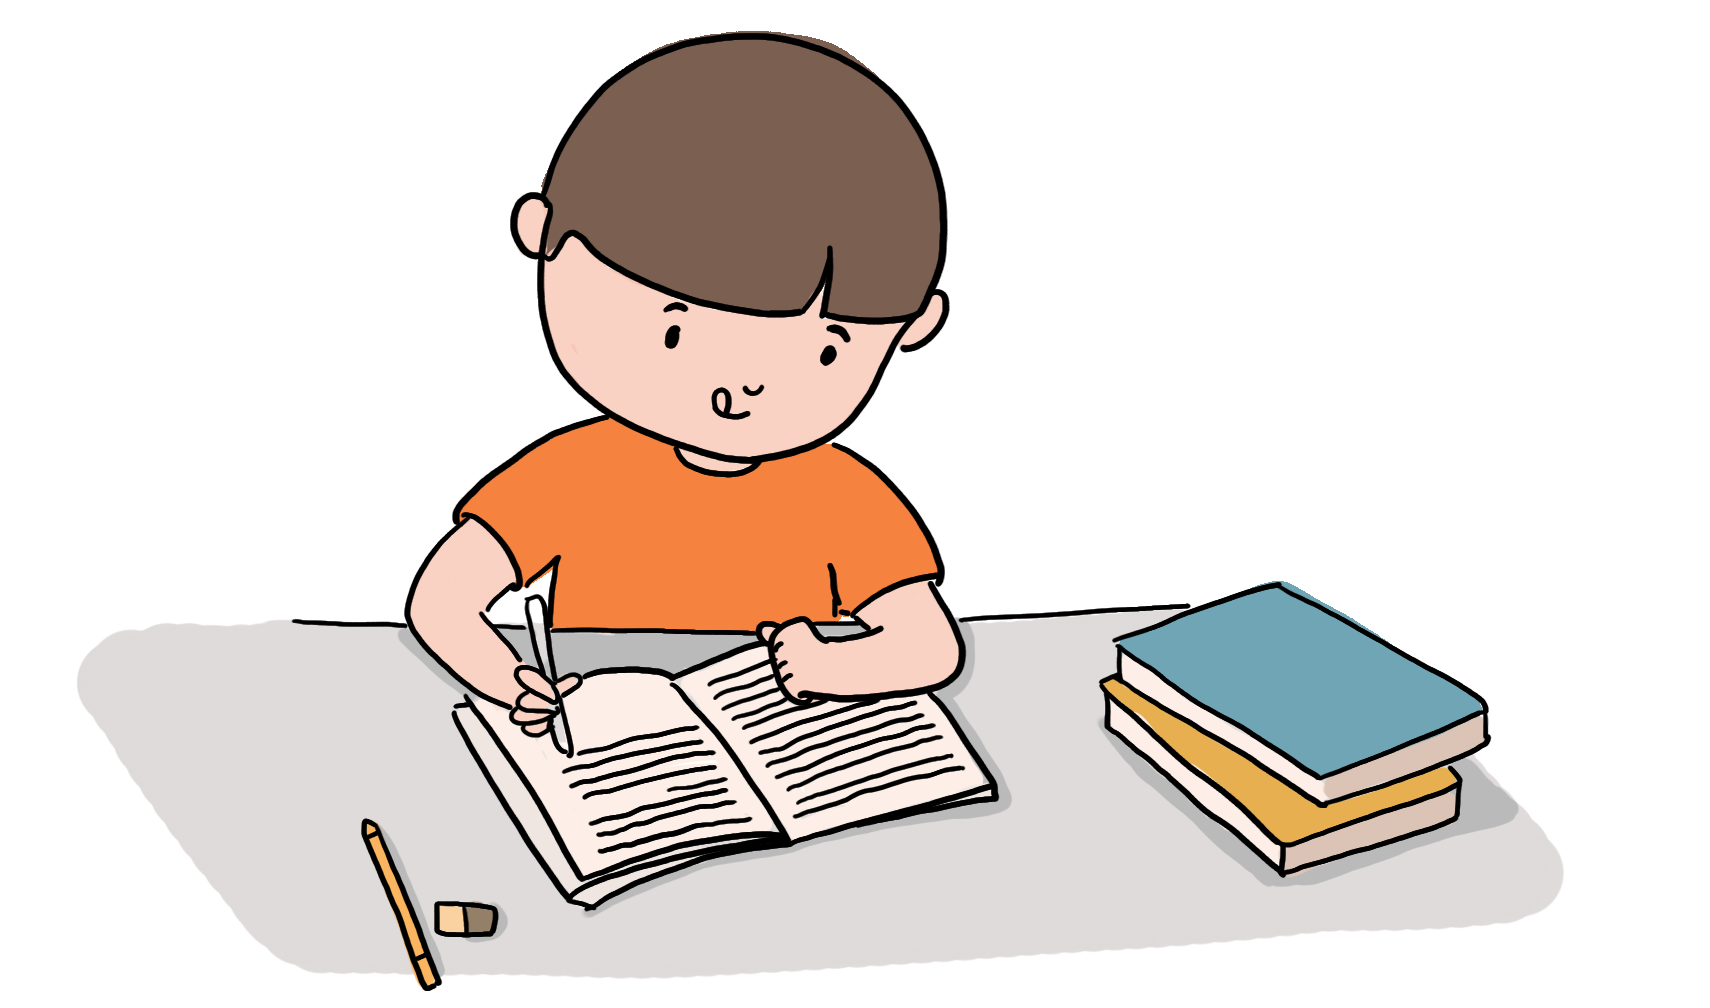
\includegraphics[width=0.95\linewidth]{Pi12_Bai1}
		\vspace*{-10pt}
	\end{figure}
	\vskip 0.1cm
	$\pmb{2.}$ Có $3$ loại kẹo để trong lọ thủy tinh với ba màu khác nhau: kẹo màu đỏ, kẹo màu vàng và kẹo màu trắng. Nếu Bình nhặt hết số kẹo màu vàng thì tổng số kẹo trong lọ ít hơn một chiếc so với $2/3$ tổng số kẹo ban đầu. Còn nếu Bình nhặt hết số kẹo đỏ, thì số kẹo còn lại trong lọ nhiều hơn $4$ chiếc so với $2/3$ tổng số kẹo ban đầu.
	\vskip 0.1cm
	Vậy ban đầu trong hai loại kẹo màu vàng và kẹo màu trắng, loại nào có nhiều và nhiều hơn bao nhiêu?
	\begin{figure}[H]
		\centering
		\vspace*{-10pt}
		\captionsetup{labelformat= empty, justification=centering}
		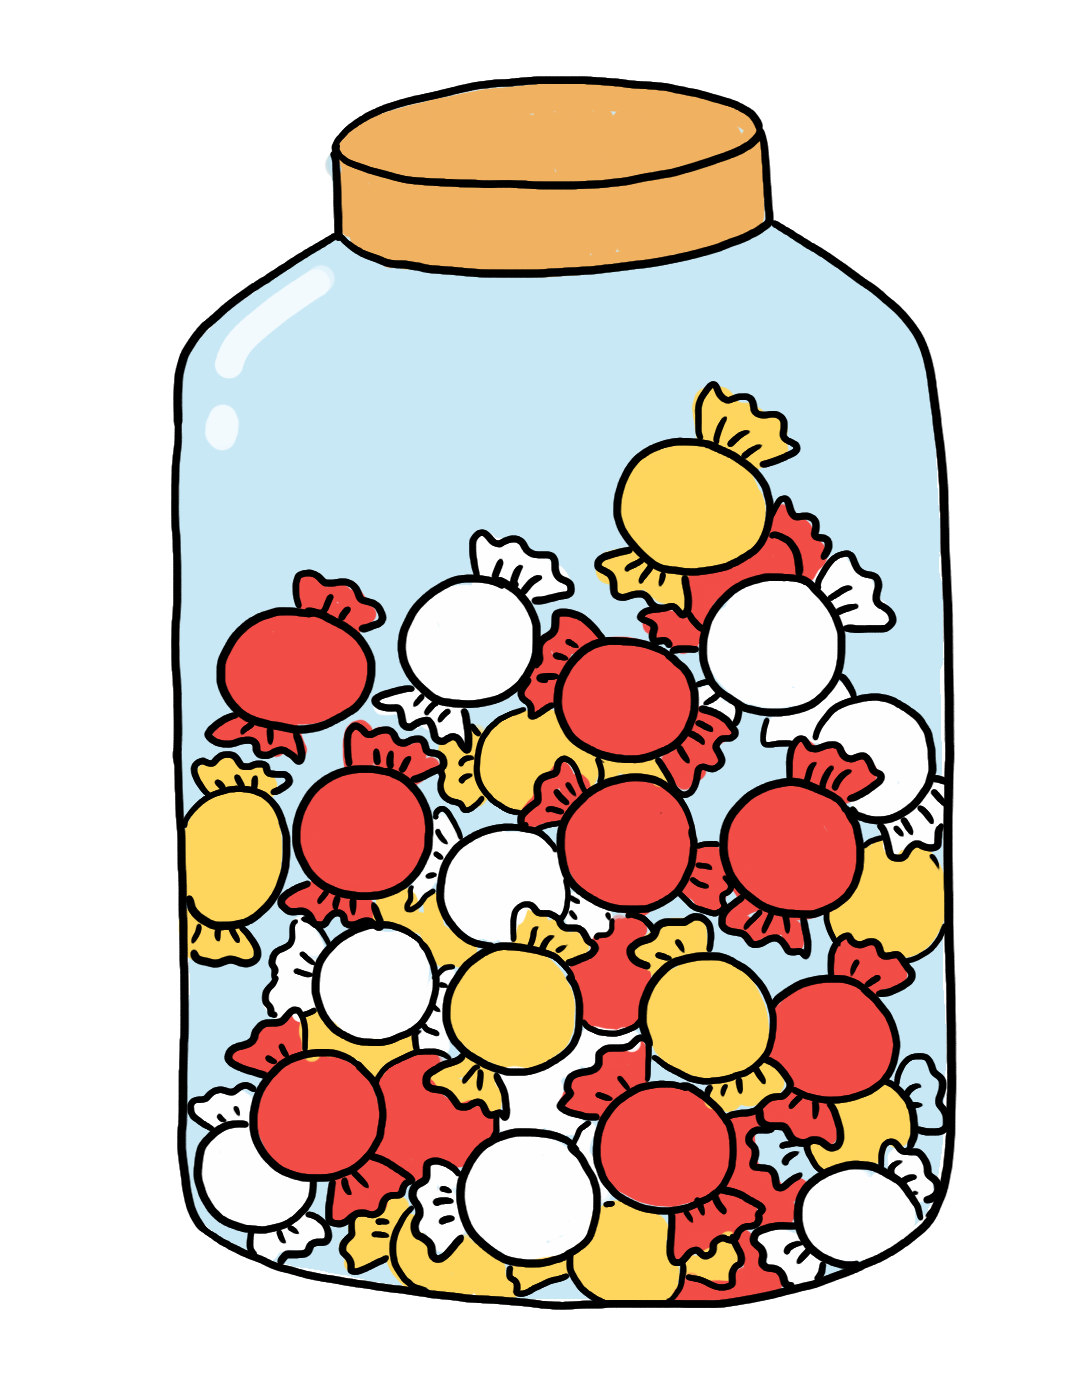
\includegraphics[width=0.45\linewidth]{Pi12_Bai2}
		\vspace*{-15pt}
	\end{figure}
	$\pmb{3.}$ $40$ bạn nhỏ nắm tay nhau xếp thành vòng tròn quanh đống lửa trại. Có tất cả $22$ bạn có nắm tay một bạn nam, và $30$ bạn có nắm tay một bạn nữ. Hỏi có tất cả bao nhiêu bạn nữ xếp trong vòng tròn quanh lửa trại ngày hôm đó?
	\begin{figure}[H]
		\centering
		\vspace*{-10pt}
		\captionsetup{labelformat= empty, justification=centering}
		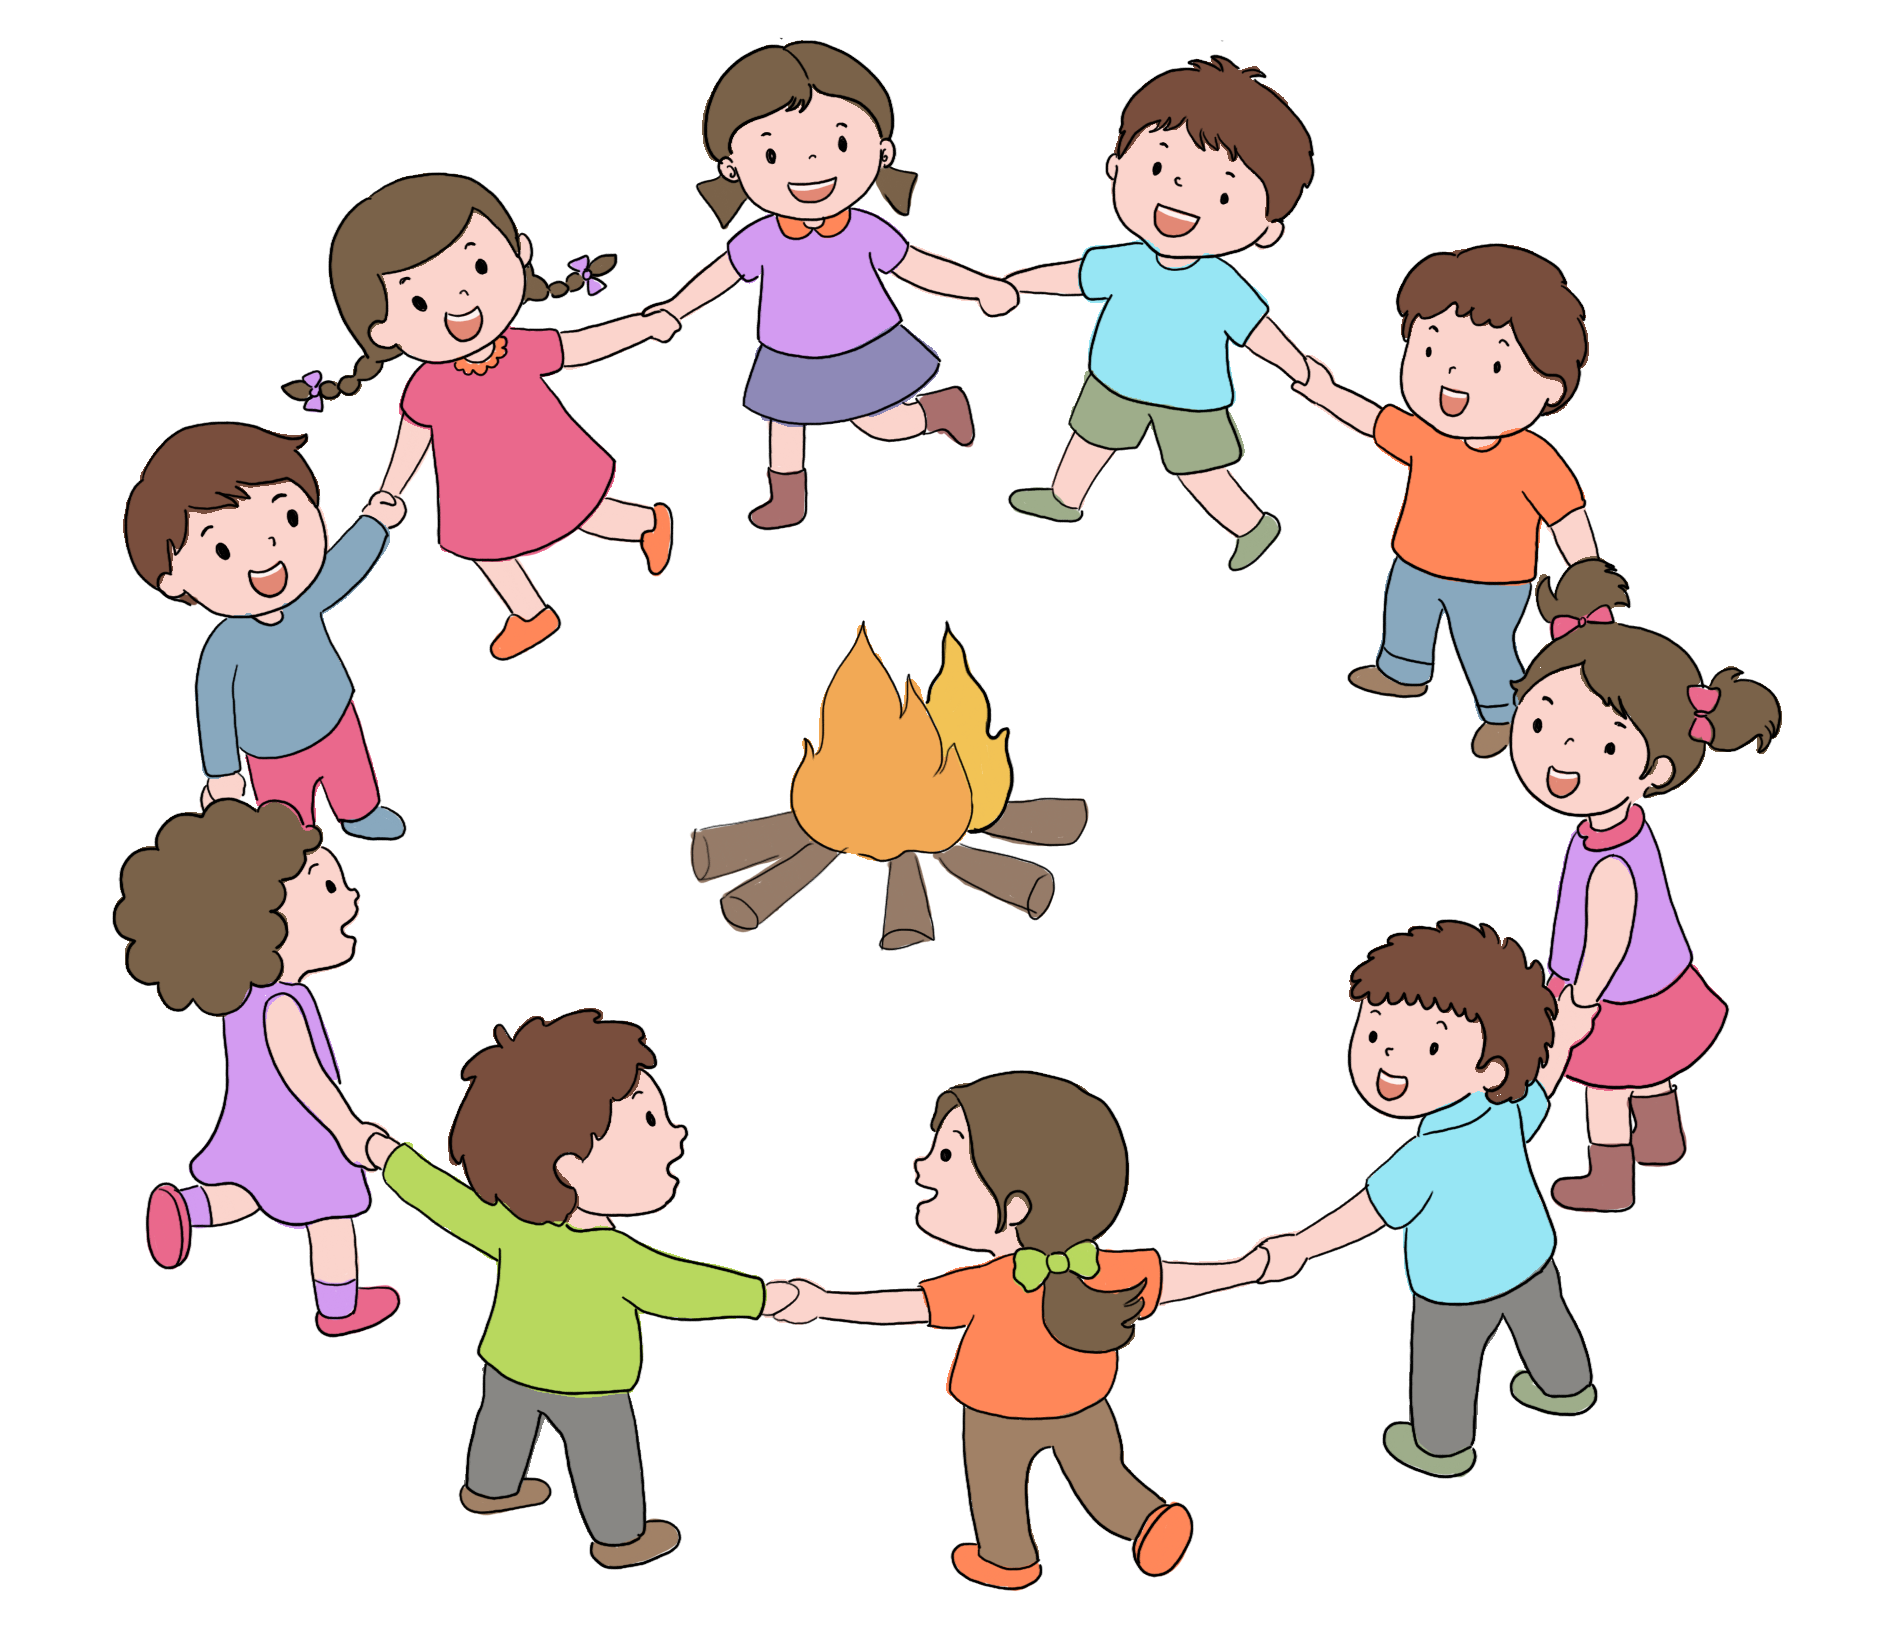
\includegraphics[width=0.9\linewidth]{Pi12_Bai3}
		\vspace*{-10pt}
	\end{figure}
	$\pmb{4.}$ Trên mặt bàn có $5$ đồng xu xếp thành hàng ngang. Đồng xu ở giữa đặt xấp còn $4$ đồng còn lại đều đặt ngửa. Mỗi một lần em được cho phép lật $3$ đồng xu đặt liền nhau tùy ý. Liệu em có thể có cách lật thế nào để cuối cùng $5$ đồng xu đều đặt xấp được không?
	\vskip 0.1cm
	Cũng câu hỏi như vậy, nếu lúc đầu đồng xu đặt xấp duy nhất là đồng xu xếp đầu hàng? Là đồng xu xếp thứ hai trong hàng?
	\begin{figure}[H]
		\centering
		\vspace*{-5pt}
		\captionsetup{labelformat= empty, justification=centering}
		
\includegraphics[width=1\linewidth]{Pi12_Bai4}
		\vspace*{-20pt}
	\end{figure}
	$\pmb{5.}$ Một lần Lý Toét diện guốc mộc loẹt quẹt ra tận chợ phiên chơi ngày cuối tuần. Khi về nhà, Lý Toét ba hoa khoe khắp làng ``Tôi là tôi gặp $15$ ông bán cây cảnh ngoài chợ nhé. Mà tôi đi lòng vòng và nghiệm thấy cứ $3$ ông bất kỳ có tổng cộng đúng $10$ cây hoa hồng. Thế là tôi lẩm nhẩm đoán được ngay $15$ ông này có tất cả bao nhiêu cây hoa hồng."
	\vskip 0.1cm
	Em có thể đoán được như Lý Toét xem $15$ ông bán cây có tất cả bao nhiêu cây hoa hồng không? Hay Lý Toét có khoác lác hay nhầm lẫn gì không nhỉ?
	\begin{figure}[H]
		\centering
%		\vspace*{1pt}
		\captionsetup{labelformat= empty, justification=centering}
		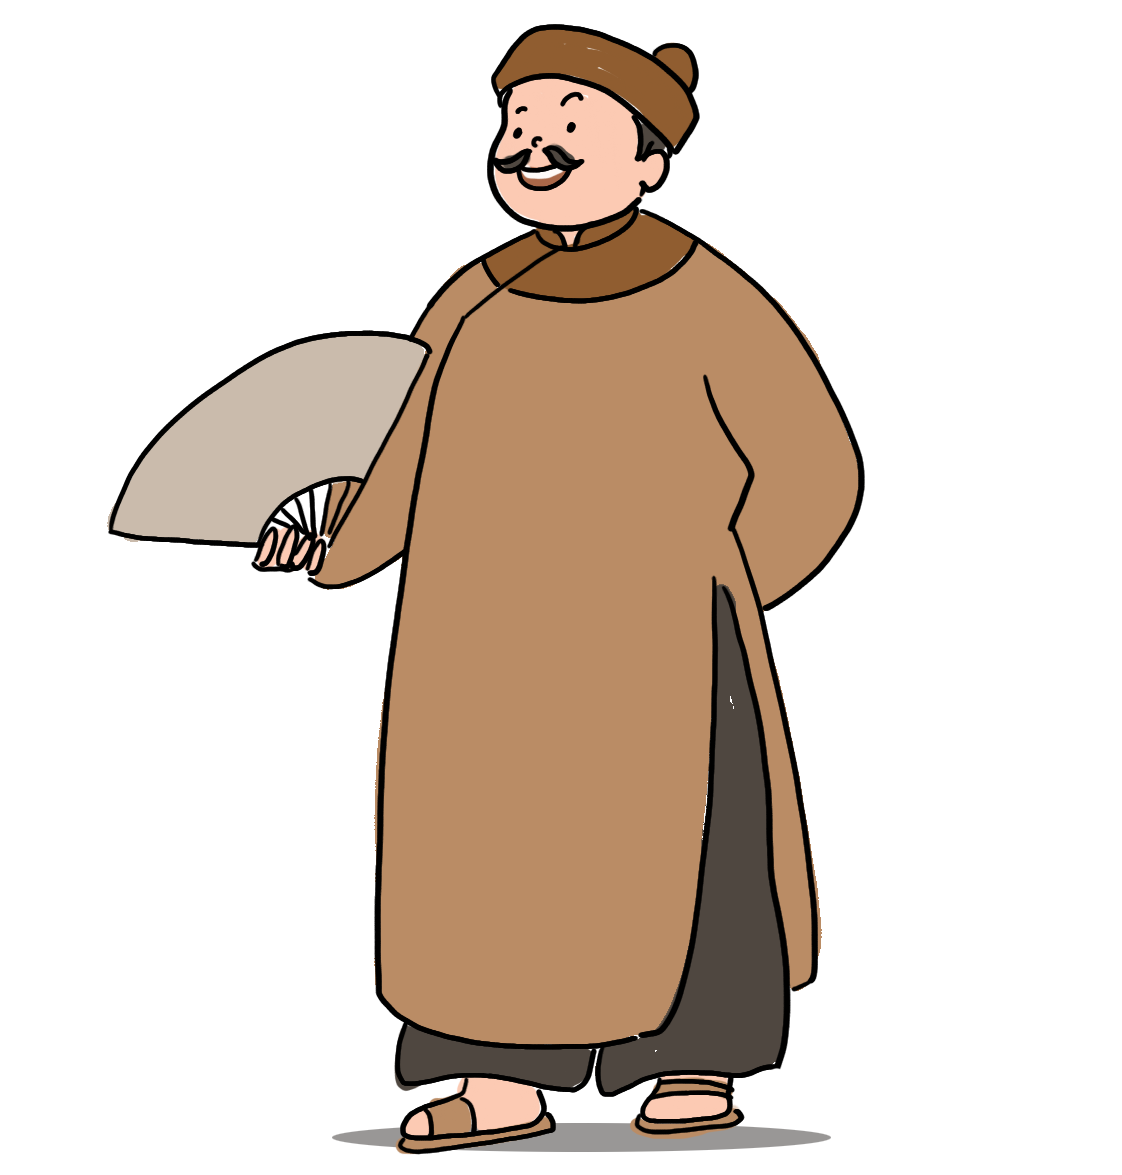
\includegraphics[width=0.58\linewidth]{Pi12_Bai5}
		\vspace*{-15pt}
	\end{figure}
	$\pmb{6.}$ Có $20$ bạn tham gia nhóm Toán ngồi xung quanh một chiếc bàn tròn. Một lúc sau các bạn nhóm Văn cũng đến, cứ xen kẽ hai bạn nhóm Toán ngồi kề nhau giờ có thêm $20$ bạn mới từ nhóm Văn. Tổng cộng có tất cả $400$ bạn từ nhóm Văn ngồi thêm quanh chiếc bàn tròn rộng đó. Thỉnh thoảng một bạn nhóm Văn lại đứng dậy và rời khỏi bàn, dắt theo hai bạn ngồi cạnh mình đi luôn. Cứ như vậy, sau một lúc thì quanh bàn số bạn nhóm Toán còn lại chỉ là $3$ bạn. Hỏi số bạn nhóm Văn còn ở lại quanh bàn lúc đó ít nhất phải là bao nhiêu?
\end{multicols}
\vspace*{-12pt}
\rule{1\linewidth}{0.1pt}
\begingroup
\AddToShipoutPicture*{\put(112,452){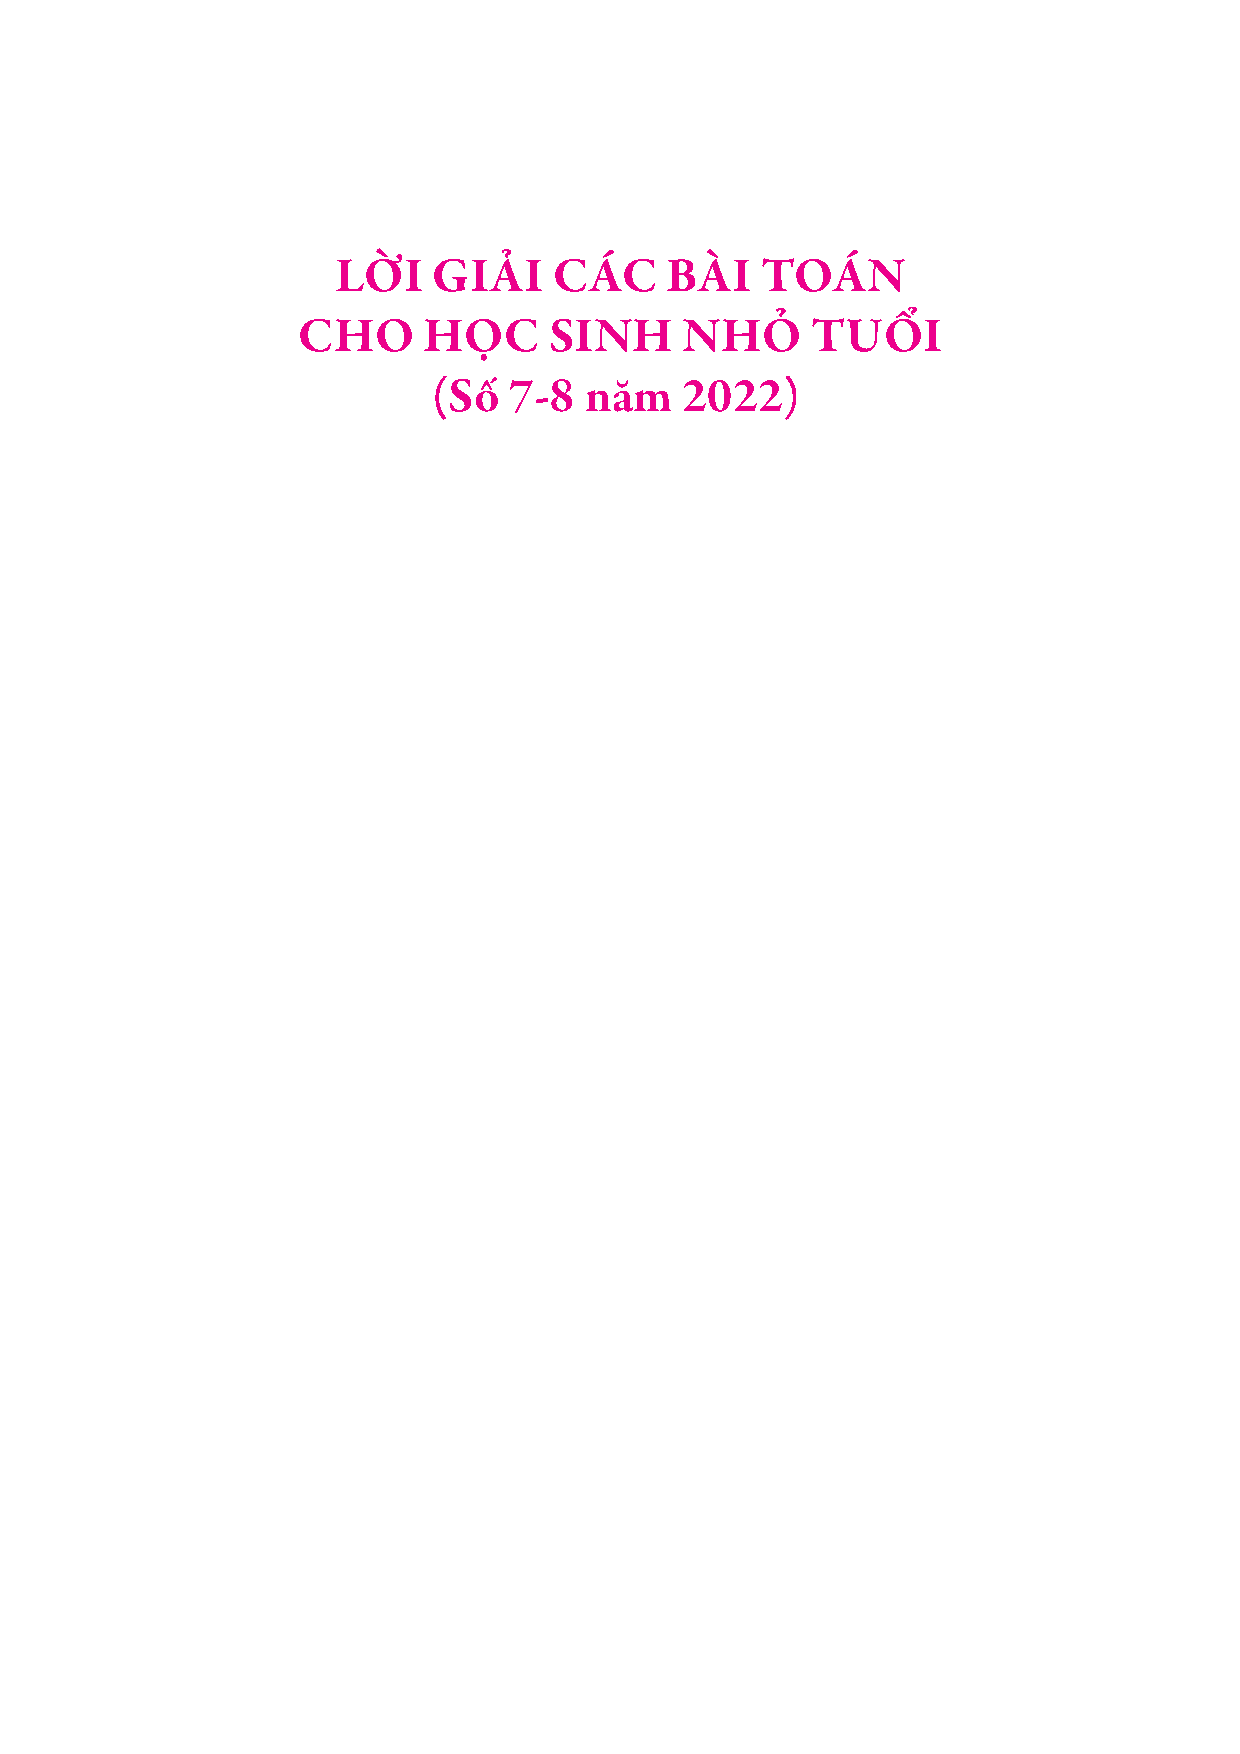
\includegraphics[scale=1]{../tieude2.pdf}}} 
\centering
\endgroup
\graphicspath{{../toancuabi/pic/}}
\vspace*{80pt}

\begin{multicols}{2}
	$\pmb{1.}$ Có $30$ bạn học sinh tham gia một cuộc thi hùng biện bằng tiếng Anh. Các bạn lần lượt chọn các câu hỏi và trả lời theo thứ tự xếp hàng. Bạn thứ nhất được $80$ điểm, bạn thứ hai được $60$ điểm, bạn thứ ba có số điểm bằng trung bình cộng của bạn thứ nhất và bạn thứ hai, bạn thứ tư có số điểm bằng trung bình cộng của ba bạn đầu tiên. Nói chung, kể từ bạn thứ ba trở đi thì  mỗi một bạn học sinh tiếp theo luôn có số điểm bằng trung bình cộng số điểm của các bạn đã thi trước đó. 
	\vskip 0.1cm
	Hỏi bạn cuối cùng, tức bạn có số thứ tự $30$, đạt được bao nhiêu điểm trong cuộc thi? 
	\begin{figure}[H]
		\centering
		\vspace*{-10pt}
		\captionsetup{labelformat= empty, justification=centering}
		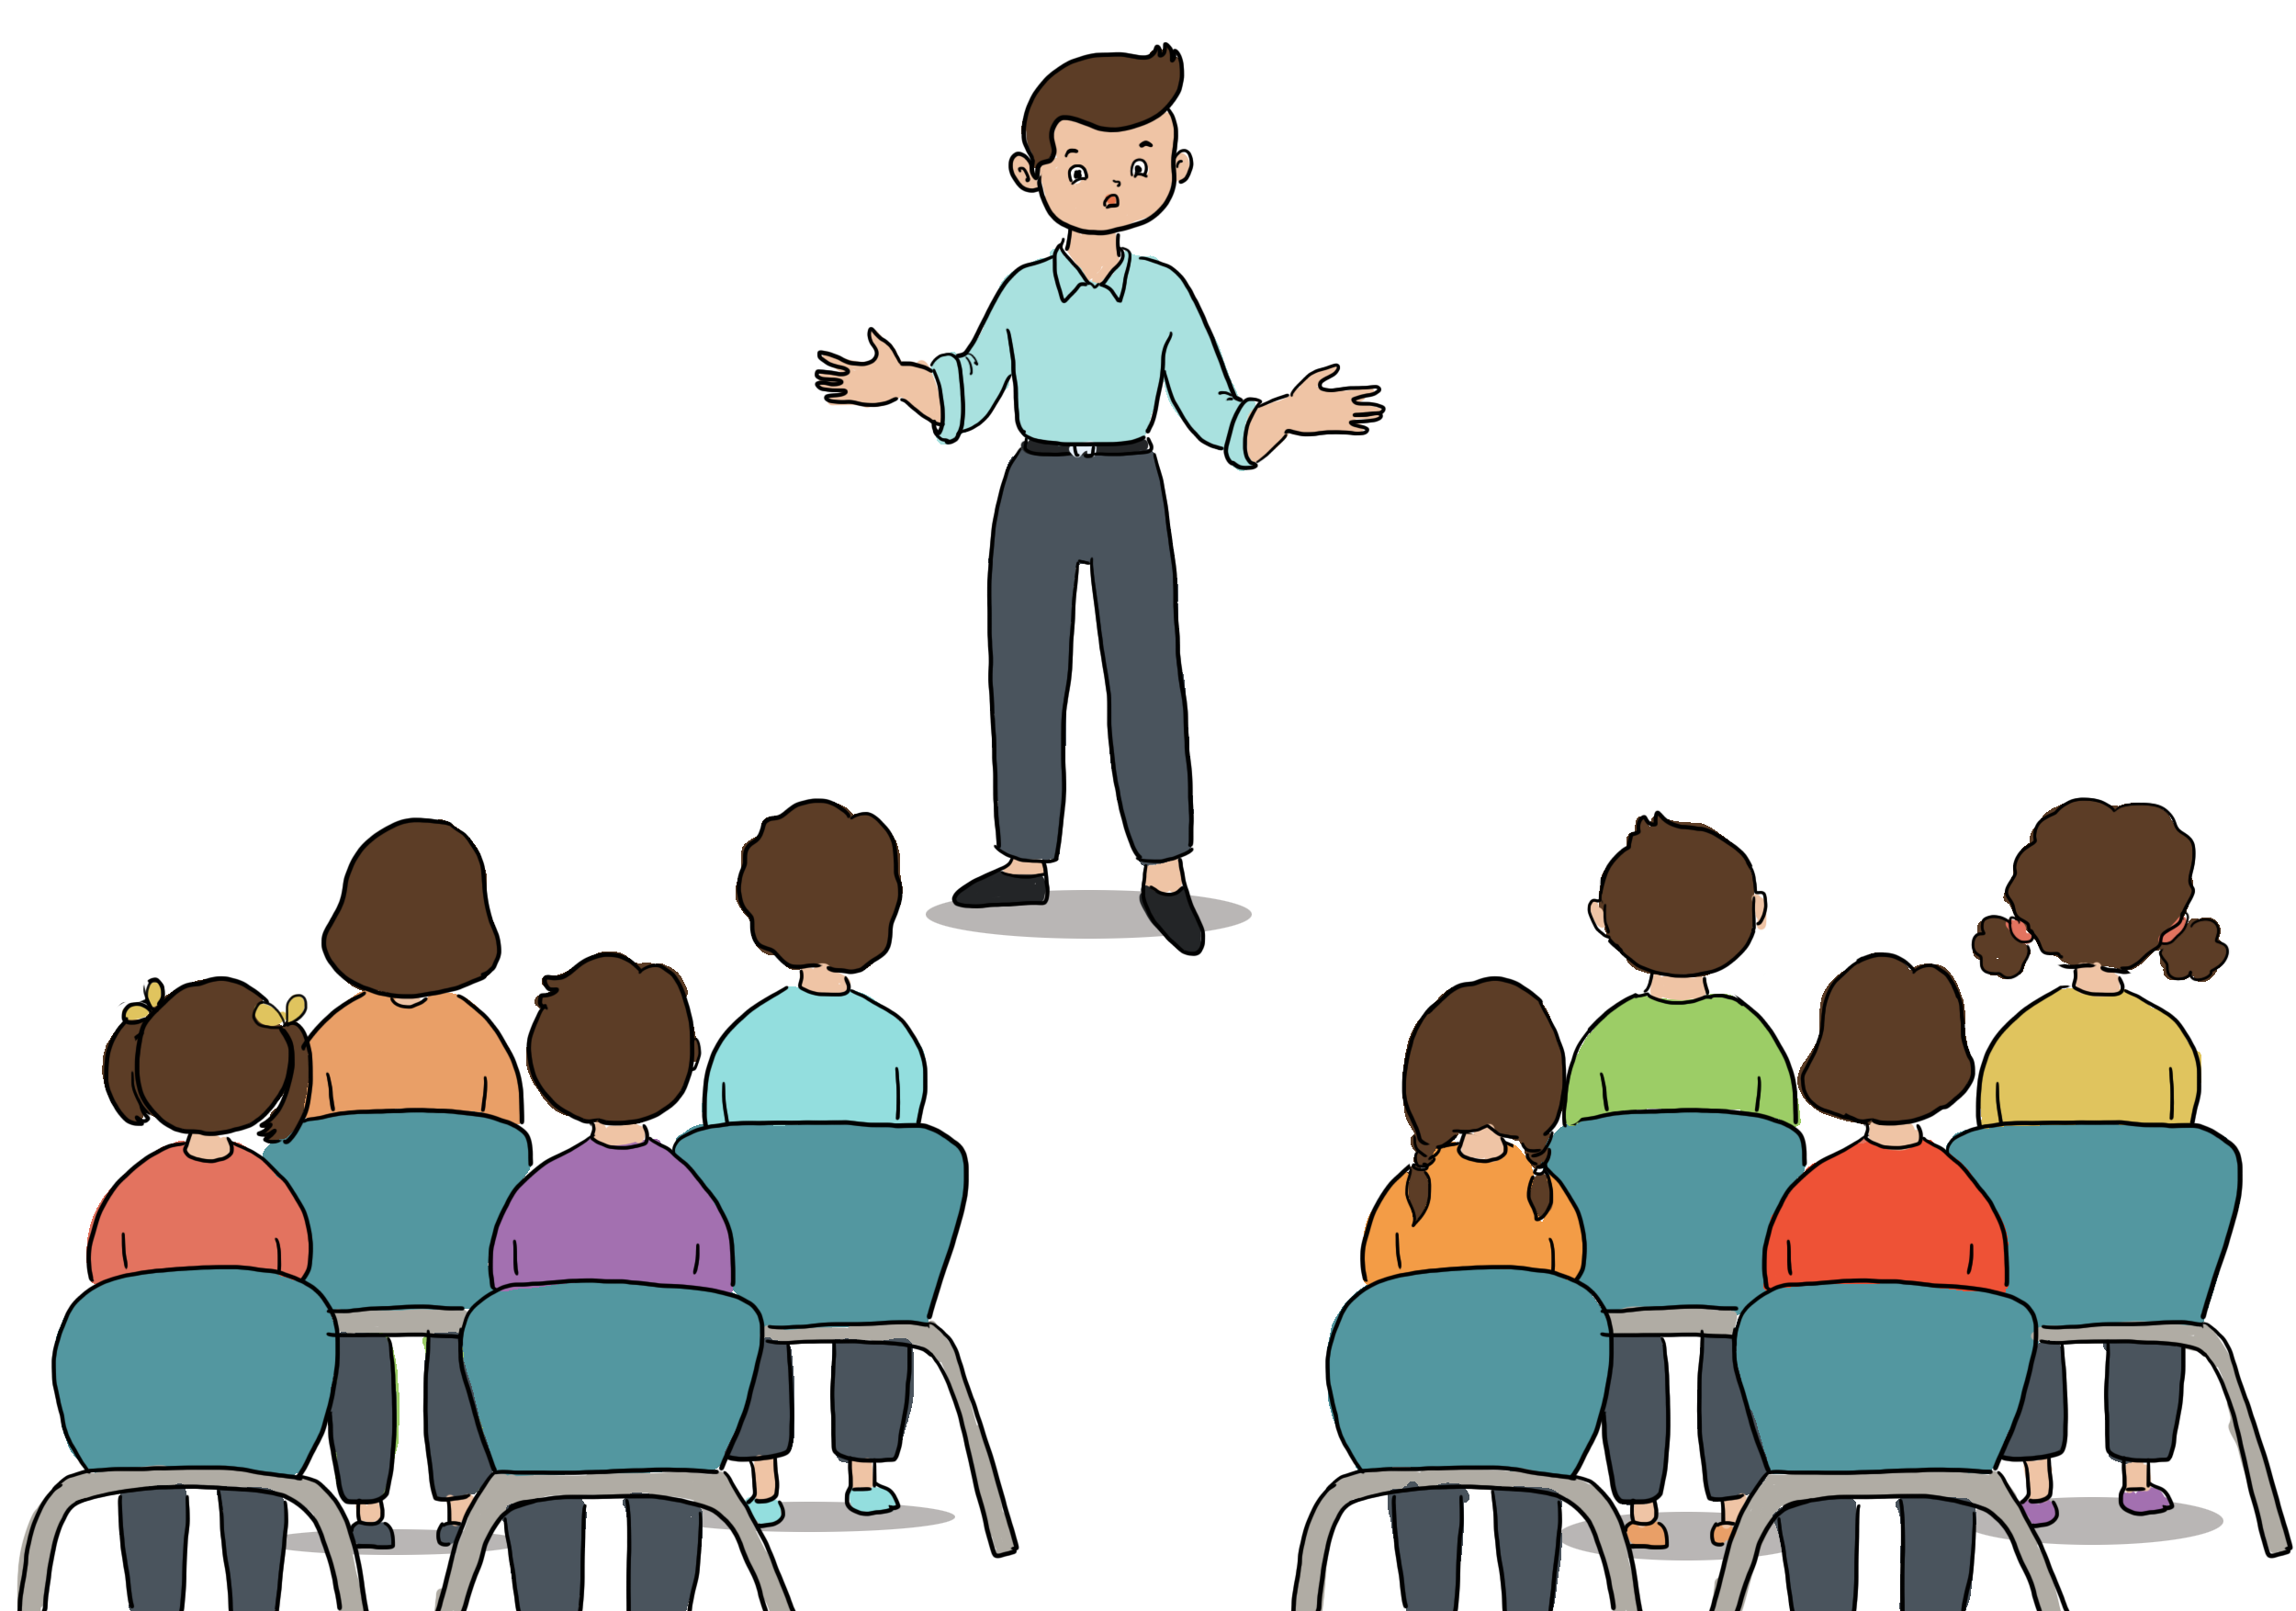
\includegraphics[width=0.92\linewidth]{bai1}
		\vspace*{-10pt}
	\end{figure}
	\textit{Lời giải.} 	Ta nhận thấy nếu mỗi bạn tiếp theo nhận được số điểm là trung bình cộng điểm số của các bạn đứng trước đó, thì trung bình cộng số điểm của các bạn luôn không thay đổi. Nếu hai bạn đầu tiên có trung bình cộng số điểm là $70$, thì kể từ bạn thứ ba, trung bình cộng số điểm của $n$ bạn đầu tiên, ($2\!<\!n\!<\!30$), luôn bằng $70$. Vì thế bạn cuối cùng cũng nhận được $70$ điểm.
	\vskip 0.1cm
	$\pmb{2.}$ Vào một ngày hè, ba bạn Yến, Vinh và Công đến hiệu kem và mỗi bạn đều lấy đủ $3$ vị: trái cây, vani và sô--cô--la (mỗi vị một cốc). Sau khi ăn xong, vì $3$ cốc cho một người là chưa đủ, nên Yến lấy thêm một cốc kem trái cây, Vinh lấy thêm một cốc kem vani và Công lấy thêm một cốc kem sô--cô--la. 
	\begin{figure}[H]
		\centering
		\vspace*{-10pt}
		\captionsetup{labelformat= empty, justification=centering}
		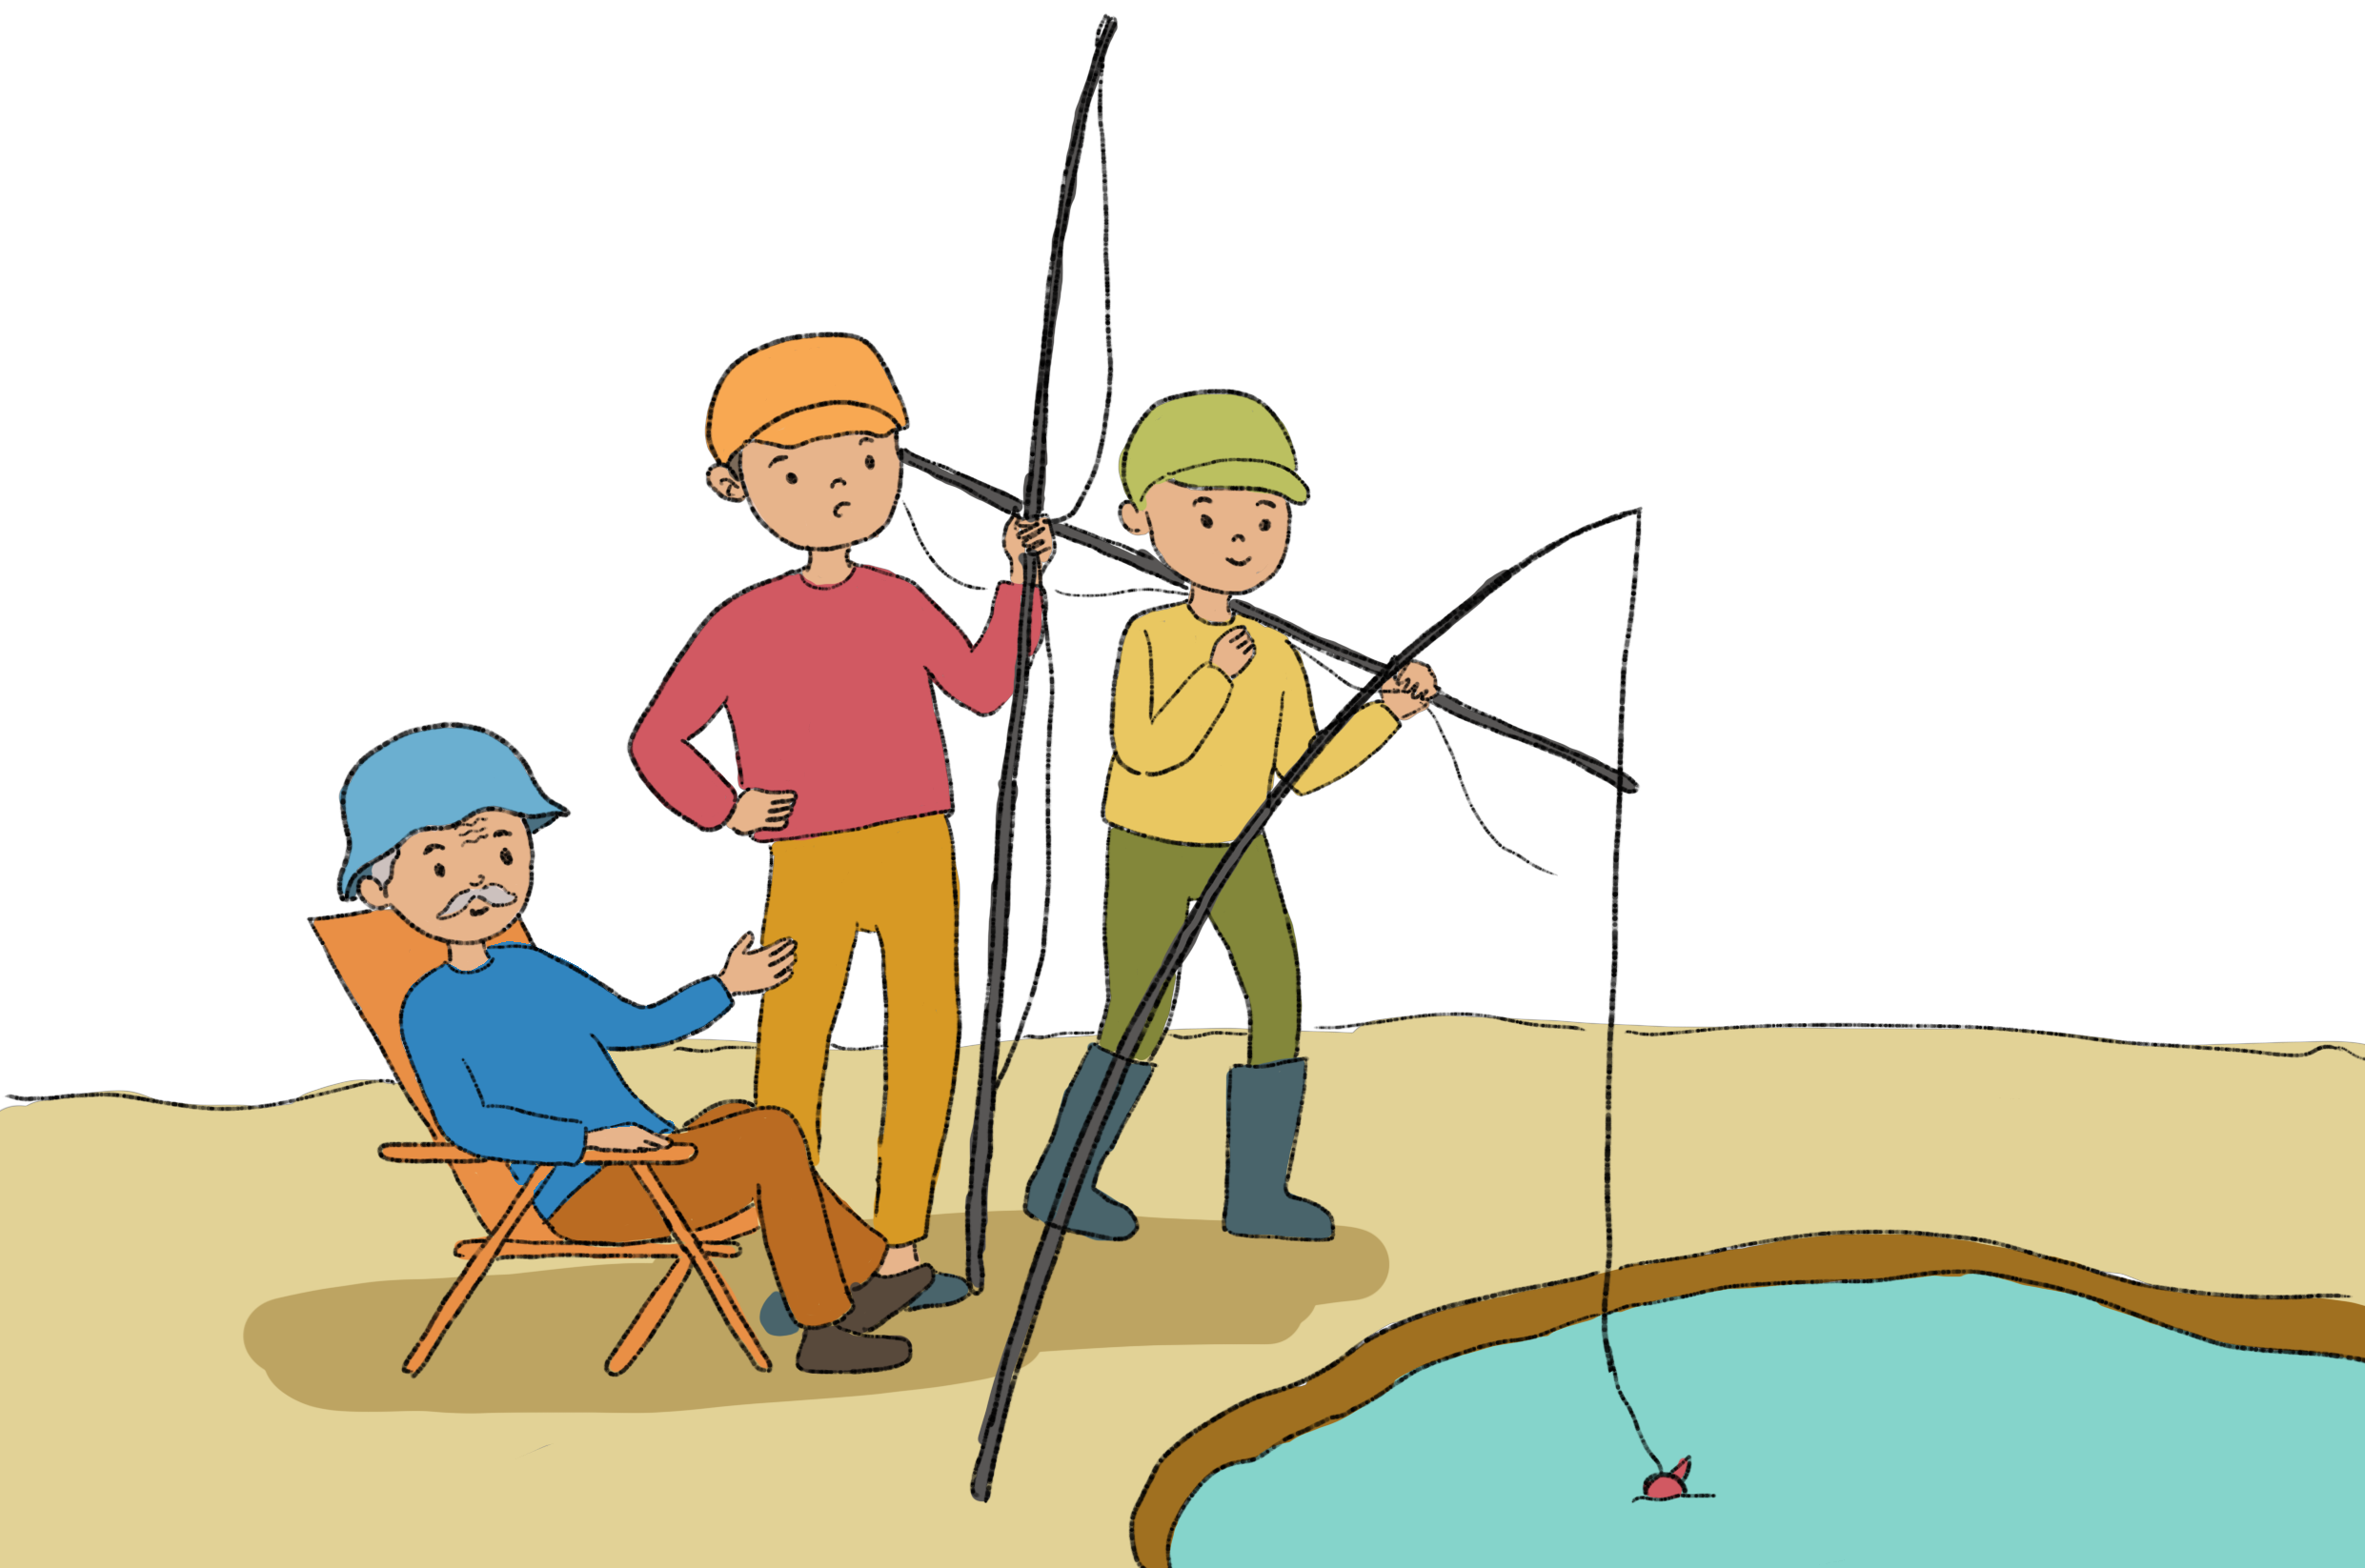
\includegraphics[width=0.92\linewidth]{bai2}
		\vspace*{-10pt}
	\end{figure}
	Lúc ra quầy thanh toán, Yến phải trả $70$ nghìn, Vinh phải trả $80$ nghìn còn Công phải trả $90$ nghìn. Hỏi mỗi vị kem có giá bao nhiêu tiền một cốc?
	\vskip 0.1cm
	\textit{Lời giải.} 	Gọi $a$ là giá tiền một cốc kem hoa quả, khi đó $a+10000$ là giá một cốc kem va--ni, còn $a+20000$ là giá một cốc kem sô--cô--la. Tổng số tiền các bạn phải trả là $70+80+90= 240$ (nghìn đồng). Tổng số này cũng bằng $4(a+a+10000+a+20000)= 12 a+ 120000$.
	\vskip 0.1cm 
	Từ đây suy ra $a= 10000$.
	\vskip 0.1cm 
	Như vậy một cốc kem hoa quả giá $10$ nghìn đồng, một cốc kem va--ni giá $20$ nghìn đồng, còn một cốc kem sô--cô--la giá $30$ nghìn đồng. 
	\vskip 0.1cm
	\textit{Cách giải khác (Cô Hồng)}: Tổng số cốc kem mỗi loại mà ba bạn Yến, Vinh, Công đã ăn là $4$ cốc, và tổng số tiền ba bạn đã trả là 
	\begin{align*}
		70 + 80 +90 = 240 \text{ (nghìn đồng).}
	\end{align*}
	Như vậy, tổng giá tiền của $1$ cốc kem hoa quả, $1$ cốc kem va--ni và $1$ cốc kem sô--cô--la là:
	\begin{align*}
		240 : 4=60 \text{ (nghìn đồng).}
	\end{align*}
	Do đó giá tiền của $1$ cốc kem hoa quả là:
	\begin{align*}
		70-60 = 10 \text{ (nghìn đồng).}
	\end{align*}
	Giá tiền của $1$ cốc kem va--ni là:
	\begin{align*}
		80-60 = 20 \text{ (nghìn đồng).}
	\end{align*}
	Và giá tiền $1$ cốc kem sô--cô--la là:
	\begin{align*}
		90-60 = 30 \text{ (nghìn đồng).}
	\end{align*}
	$\pmb{3.}$ Ba chú khỉ con dễ thương có tên là Bibi, Bobo, và Bubu được diện áo và giày thật đẹp để quay video đăng YouTube. Các chú được mặc ba chiếc áo có các màu khác nhau là đỏ, xanh lá cây và xanh lơ. Giày của ba chú cũng có ba màu như thế, mỗi chú mang một màu. Bibi thì diện áo và giày có cùng màu. Bobo lại không thích màu đỏ, nên cả giày và áo đều không phải đỏ. Bubu thì mang giày xanh lá cây, còn áo lại khác màu giày. Vậy các chú khỉ đã mặc áo và đi giày có màu như thế nào nhỉ?
	\begin{figure}[H]
		\centering
		\vspace*{-5pt}
		\captionsetup{labelformat= empty, justification=centering}
		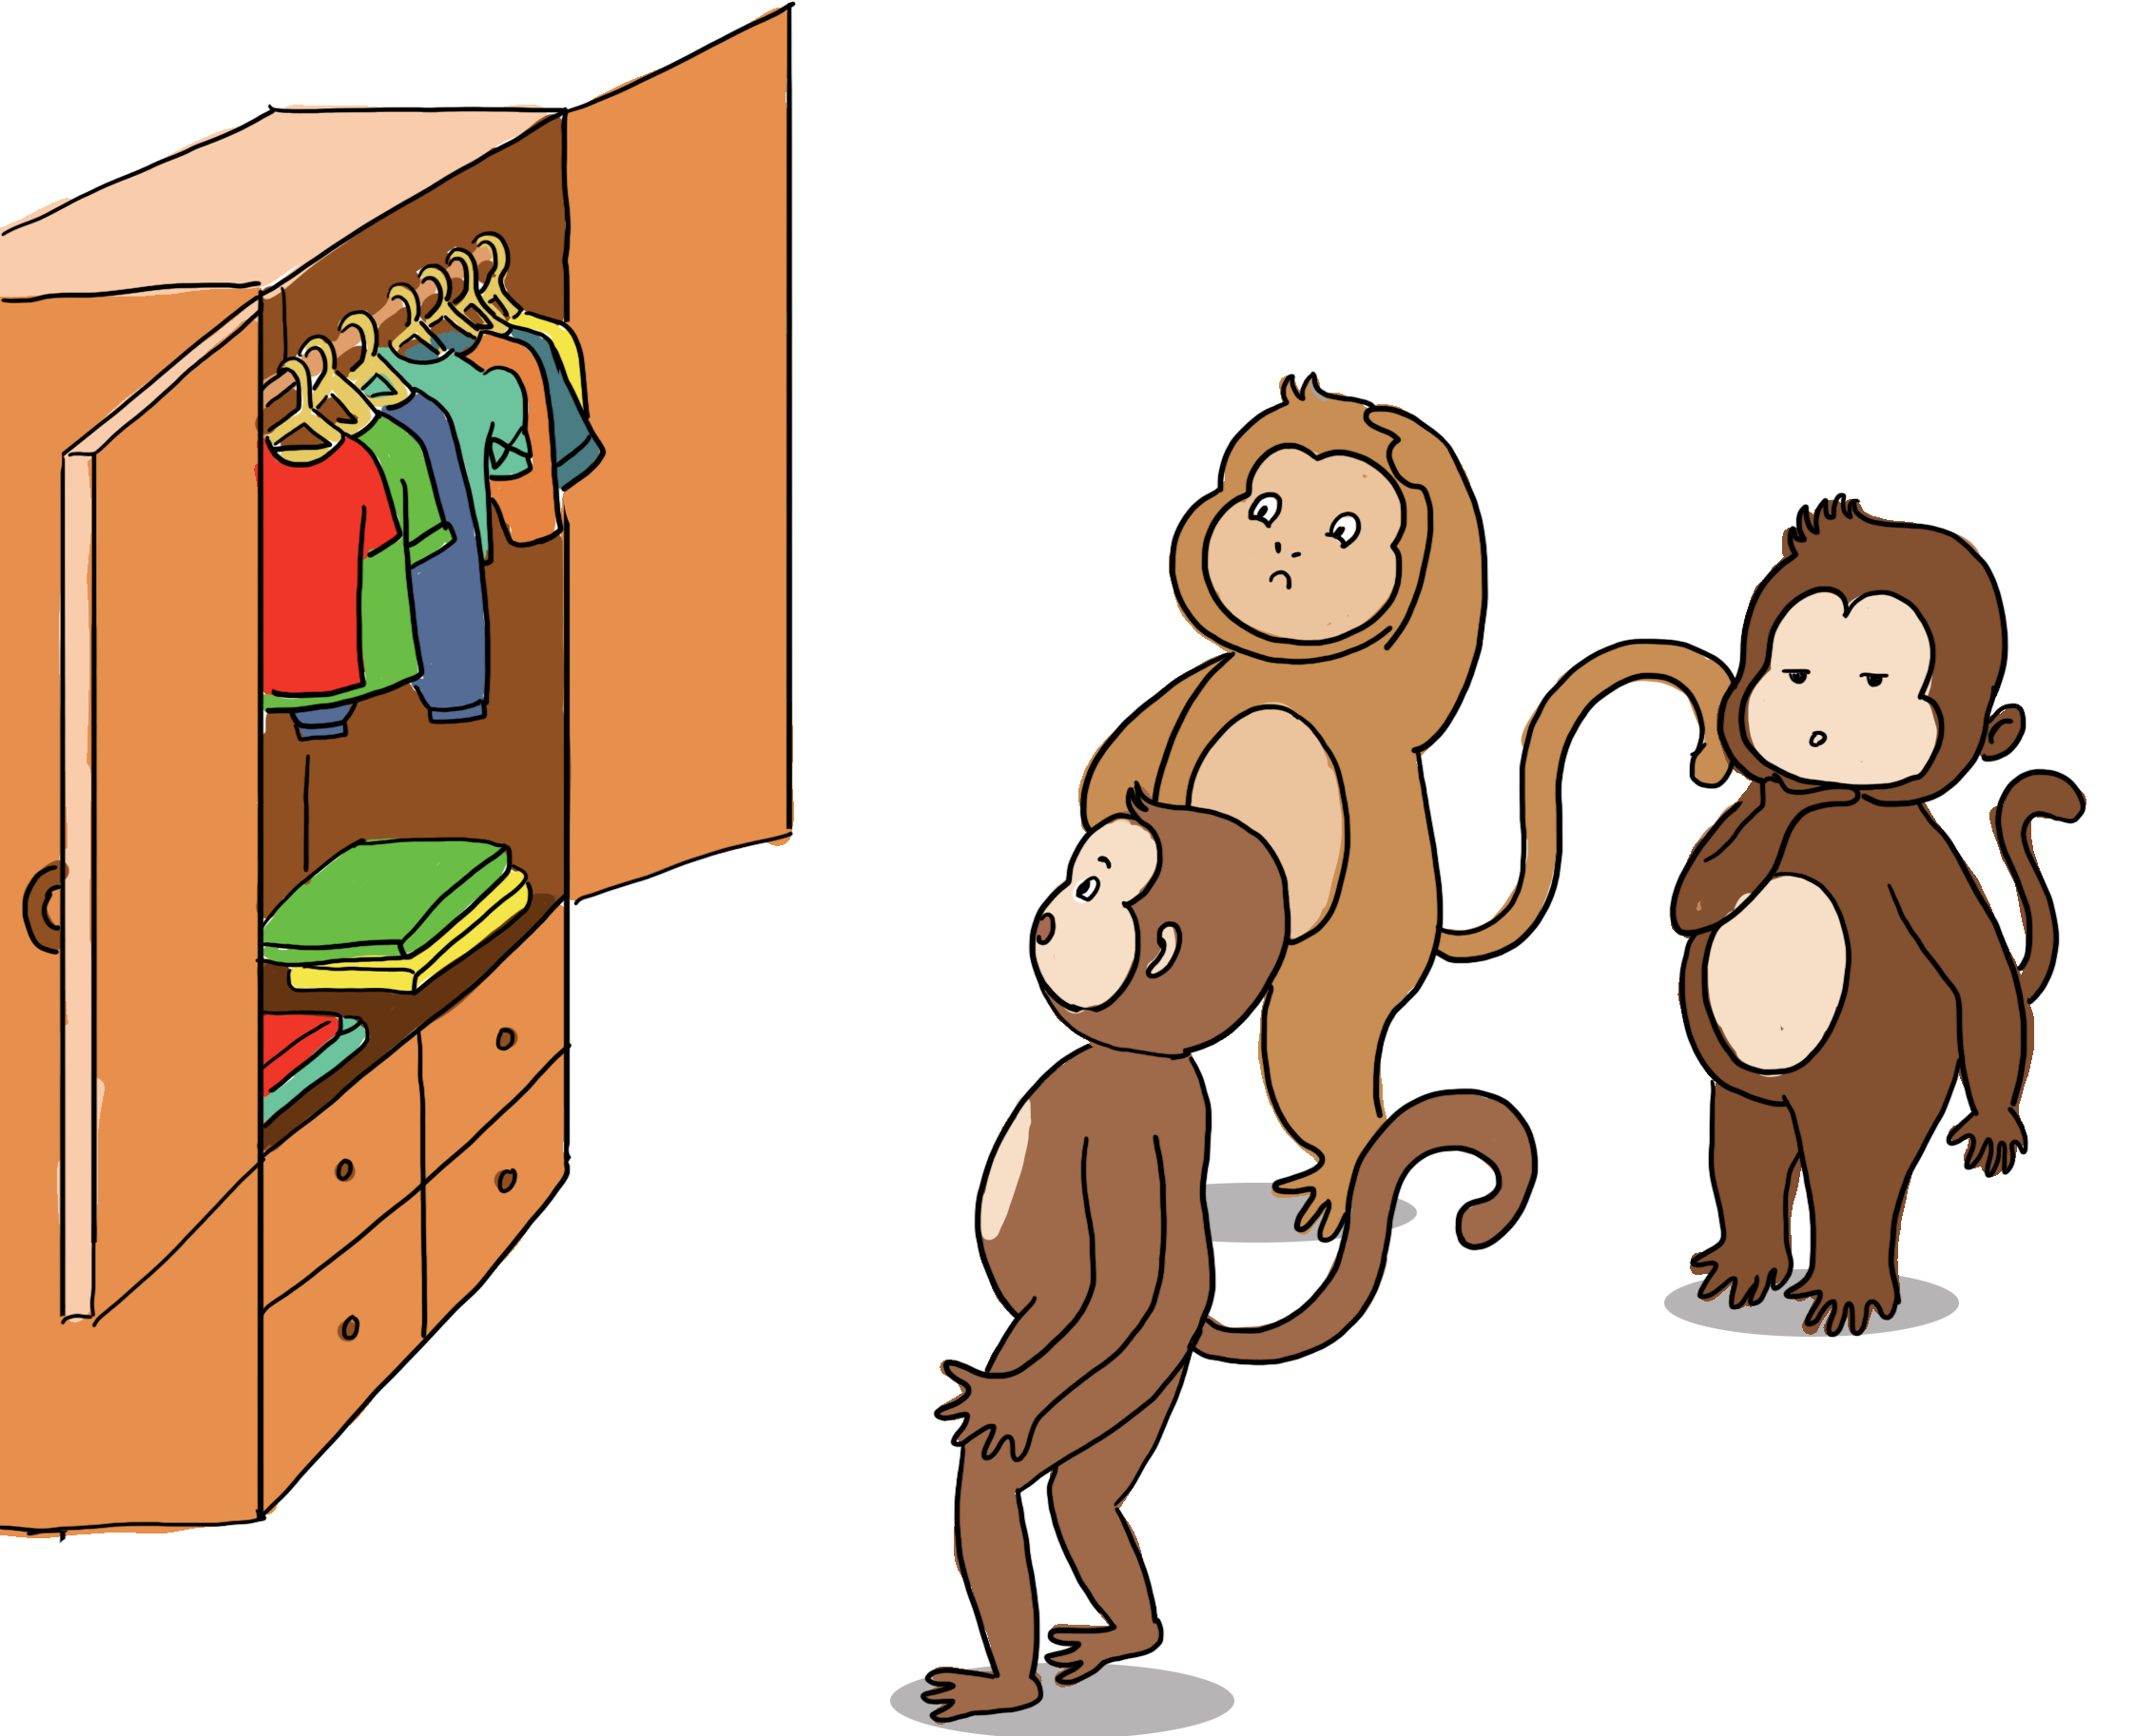
\includegraphics[width=1\linewidth]{bai3}
		\vspace*{-18pt}
	\end{figure}
	\textit{Lời giải.} Các em thấy ngay chỉ có Bibi mới mang giày màu đỏ, vì ngoài chú ta ra không có chú khỉ nào còn lại có thể mang giày đỏ. Vì thế Bibi mặc cả bộ áo và giày đều đỏ. Và suy ra Bubu phải mặc áo màu xanh lơ. Cuối cùng, ta thấy Bobo mặc áo xanh lá cây và đi giày màu xanh lơ. Các chú trông thật vui mắt khi lên hình, phải không nào các em?
	\vskip 0.1cm
	$\pmb{4.}$ Để chuẩn bị cho cuộc đua xe đạp sắp diễn ra, sáng sớm Gấu con đã mang xe ra tập luyện. Lúc đi tốc độ của Gấu con là $15$ dặm/giờ. Do đường khá đông nên chiều trở về dù vẫn đi trên con đường đó nhưng Gấu con chỉ di chuyển với tốc độ $10$ dặm/giờ. Hỏi trên cả quãng đường lúc đi và về vận tốc trung bình của Gấu con là bao nhiêu?
	\begin{figure}[H]
		\centering
		\vspace*{-5pt}
		\captionsetup{labelformat= empty, justification=centering}
		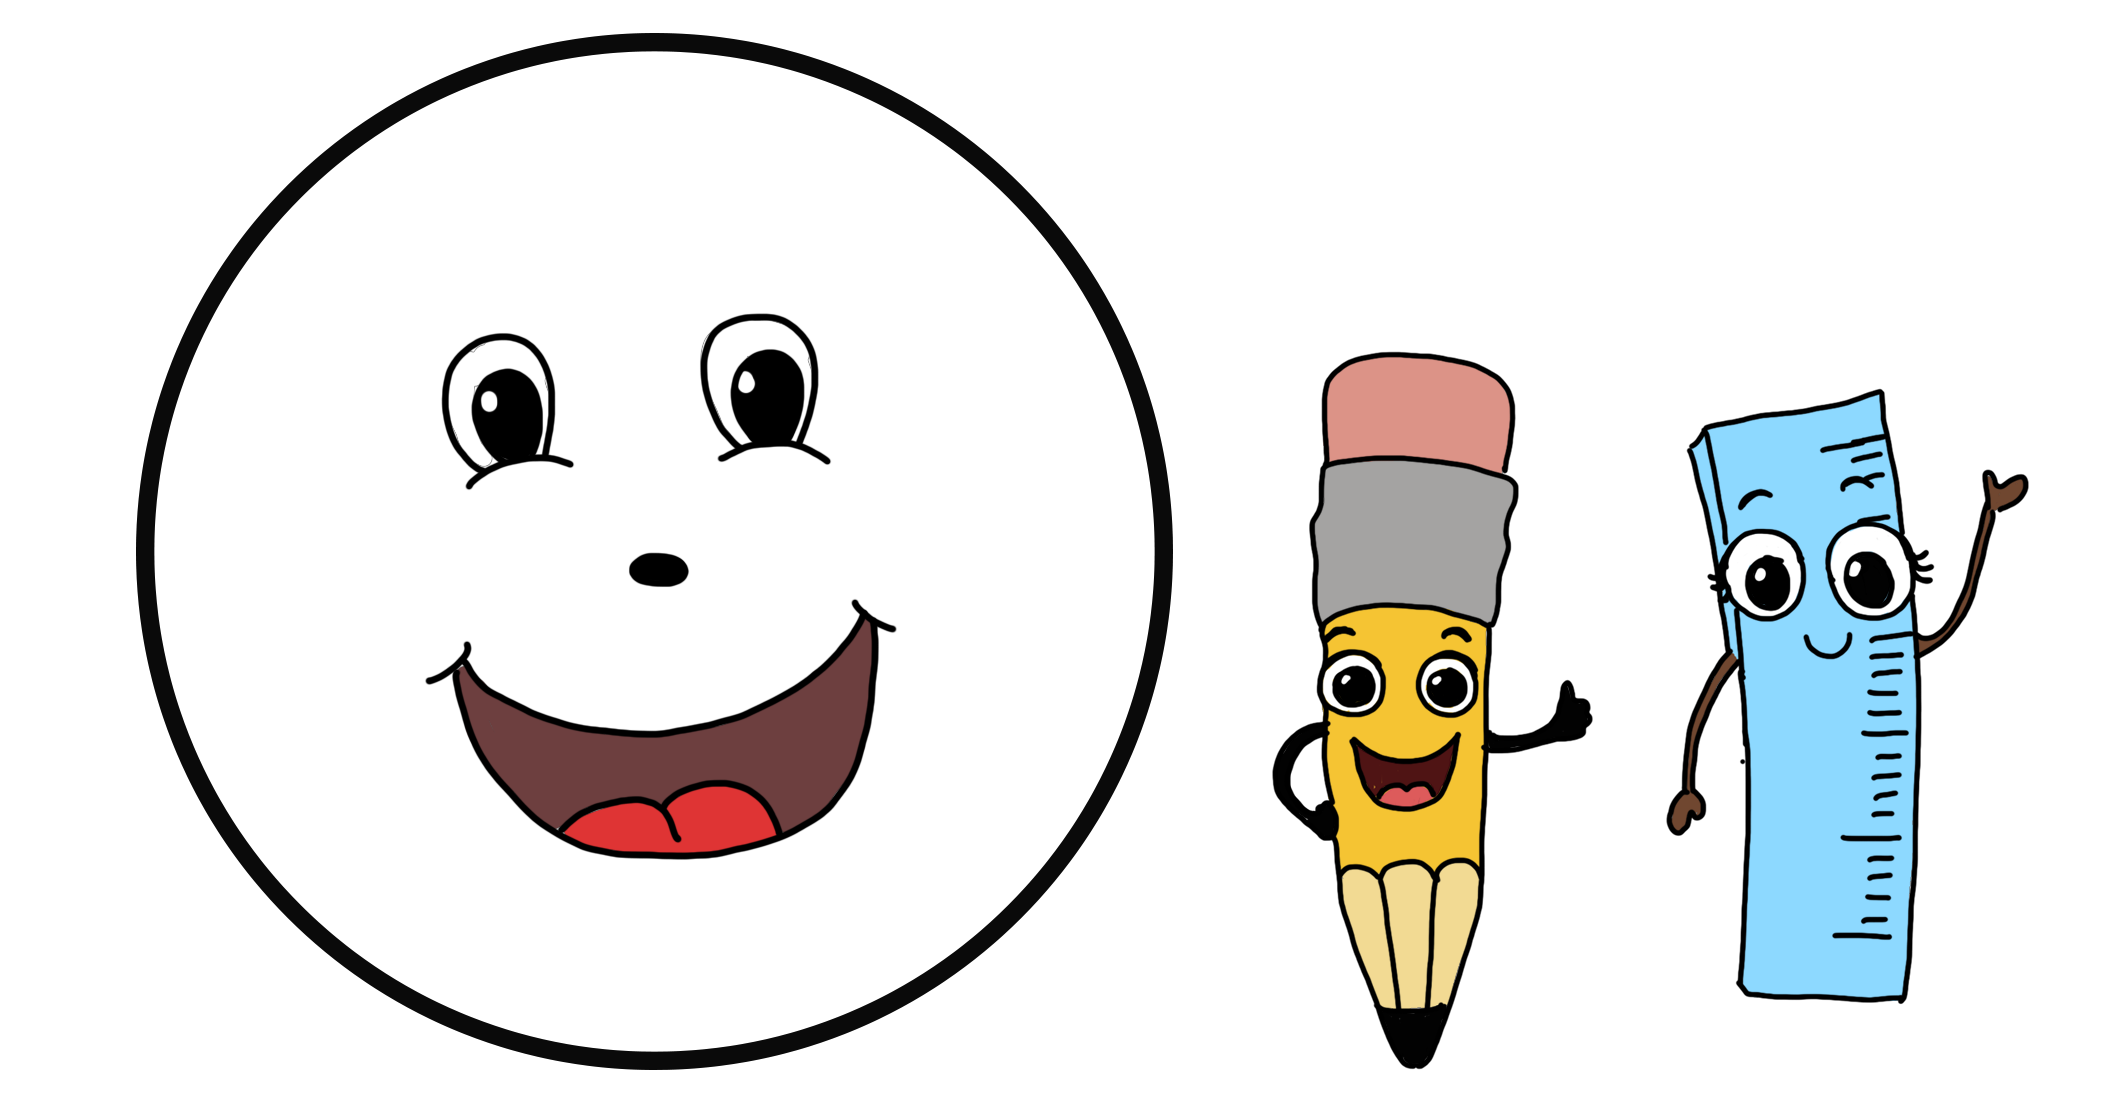
\includegraphics[width=1\linewidth]{bai4}
		\vspace*{-18pt}
	\end{figure}
	\textit{Lời giải.} 	Nhận thấy nếu quãng đường có khác nhau cũng ko ảnh hưởng tới kết quả tính vận tốc trung bình. Giả sử quãng đường là $30$ dặm, thời gian lúc đi của Gấu là:
	\begin{align*}
		30:15 =  2 \text{ (giờ).}
	\end{align*}
	Thời gian lúc về là
	\begin{align*}
		30:10 = 3 \text{ (giờ).}
	\end{align*}
	Vậy Gấu con đã đi tổng cộng $60$ dặm trong $5$ giờ nên vận tốc trung bình là
	\begin{align*}
		60:5 = 12 \text{ (dặm/giờ).}
	\end{align*}
	$\pmb{5.}$ Trên bàn có một đống đá cuội gồm $1001$ viên. Người ta lấy ra một viên đá và chia đống đá ra  thành hai đống mới, sao cho mỗi đống có ít nhất $3$ viên. Bây giờ, trong mỗi một đống đá mới, người ta lại lấy ra một viên đá và chia đống đó ra thành hai đống mới, và cứ tiếp tục như vậy. Hỏi có thể lấy các viên đá sao cho sau một số lần lấy, trên bàn chỉ còn toàn các đống đá mà mỗi đống có đúng $3$ viên được hay không?
	\begin{figure}[H]
		\centering
		\vspace*{-5pt}
		\captionsetup{labelformat= empty, justification=centering}
		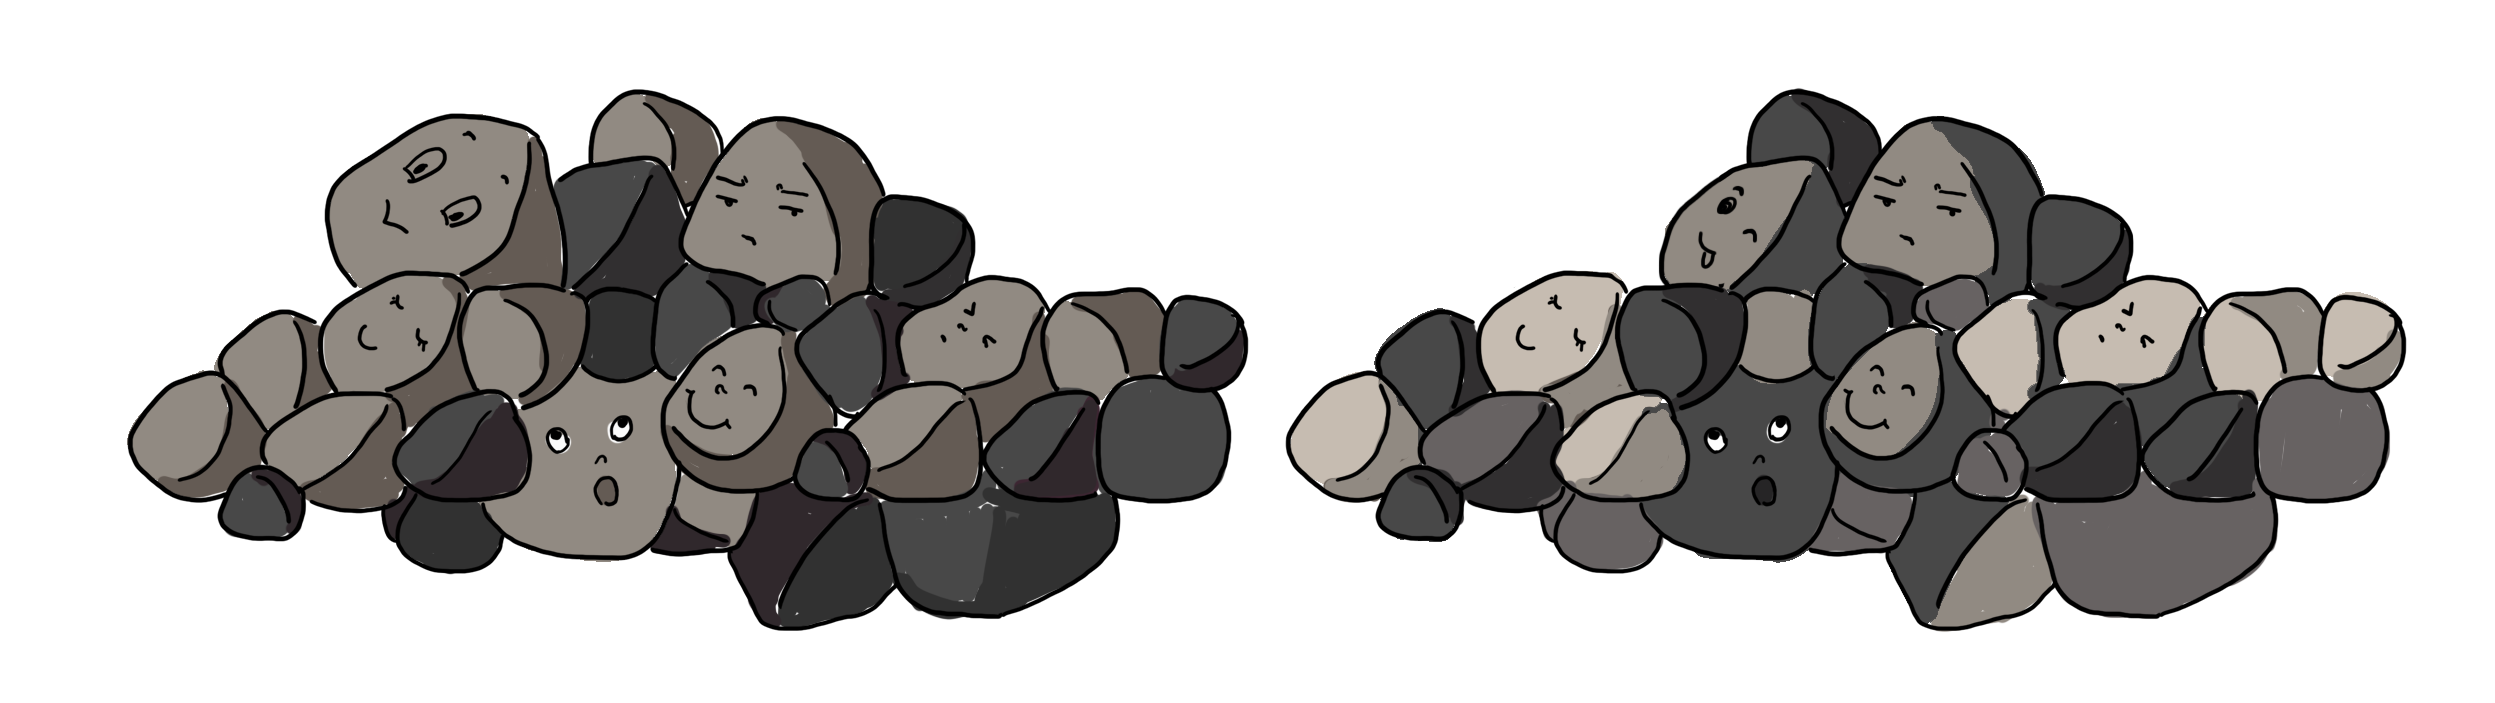
\includegraphics[width=1\linewidth]{bai5}
		\vspace*{-15pt}
	\end{figure}
	\textit{Lời giải.} 	Ta nhận thấy sau mỗi một bước, số đá trên bàn giảm đi $1$ viên nhưng số đống đá lại tăng thêm $1$. Vì vậy tổng số các viên đá và số các đống đá ở trên bàn không thay đổi sau mỗi lần nhặt bớt đi viên đá. Ban đầu tổng số này là $1001+1=1002$ không chia hết cho $4$. Vì thế, ta không thể nhận được tình huống khi trên bàn chỉ còn toàn các đống đá, mỗi đống có đúng $3$ viên, vì khi đó tổng số này sẽ bằng $3k+k=4k$ (chia hết cho $4$), ở đó $k$ là số các đống đá lúc đó ở trên mặt bàn. 
	\vskip 0.1cm
 	$\pmb{6.}$ Thạch Sanh chuẩn bị lên đường tiêu diệt Mãng xà -- con quái vật có tận $3$ cái đầu và $3$ cái đuôi gớm ghiếc. Ngài Thần Miếu đưa cho chàng một bảo bối và dặn dò: ``Đây là chiếc gươm thần thiêng liêng. Bằng một nhát gươm, con có thể chém đứt được một cái đầu, hoặc là hai cái đầu, hoặc là một cái đuôi, hoặc là hai cái đuôi của con Mãng xà. Nhưng con nên nhớ, nếu con chỉ chém đứt một cái đầu, thì một cái đầu khác của nó sẽ mọc lên, nếu chỉ chém đứt một cái đuôi, thì hai cái đuôi khác lại mọc ra, nếu chém đứt hai cái đuôi thì một cái đầu khác lại mọc ra, còn nếu con chém đứt được hai cái đầu thì không có gì mọc ra thêm nữa". Vậy Thạch Sanh có thể chém đứt tất cả đầu và đuôi của con Mãng xà sau bao nhiêu nhát gươm?
	\begin{figure}[H]
		\centering
		\vspace*{-5pt}
		\captionsetup{labelformat= empty, justification=centering}
		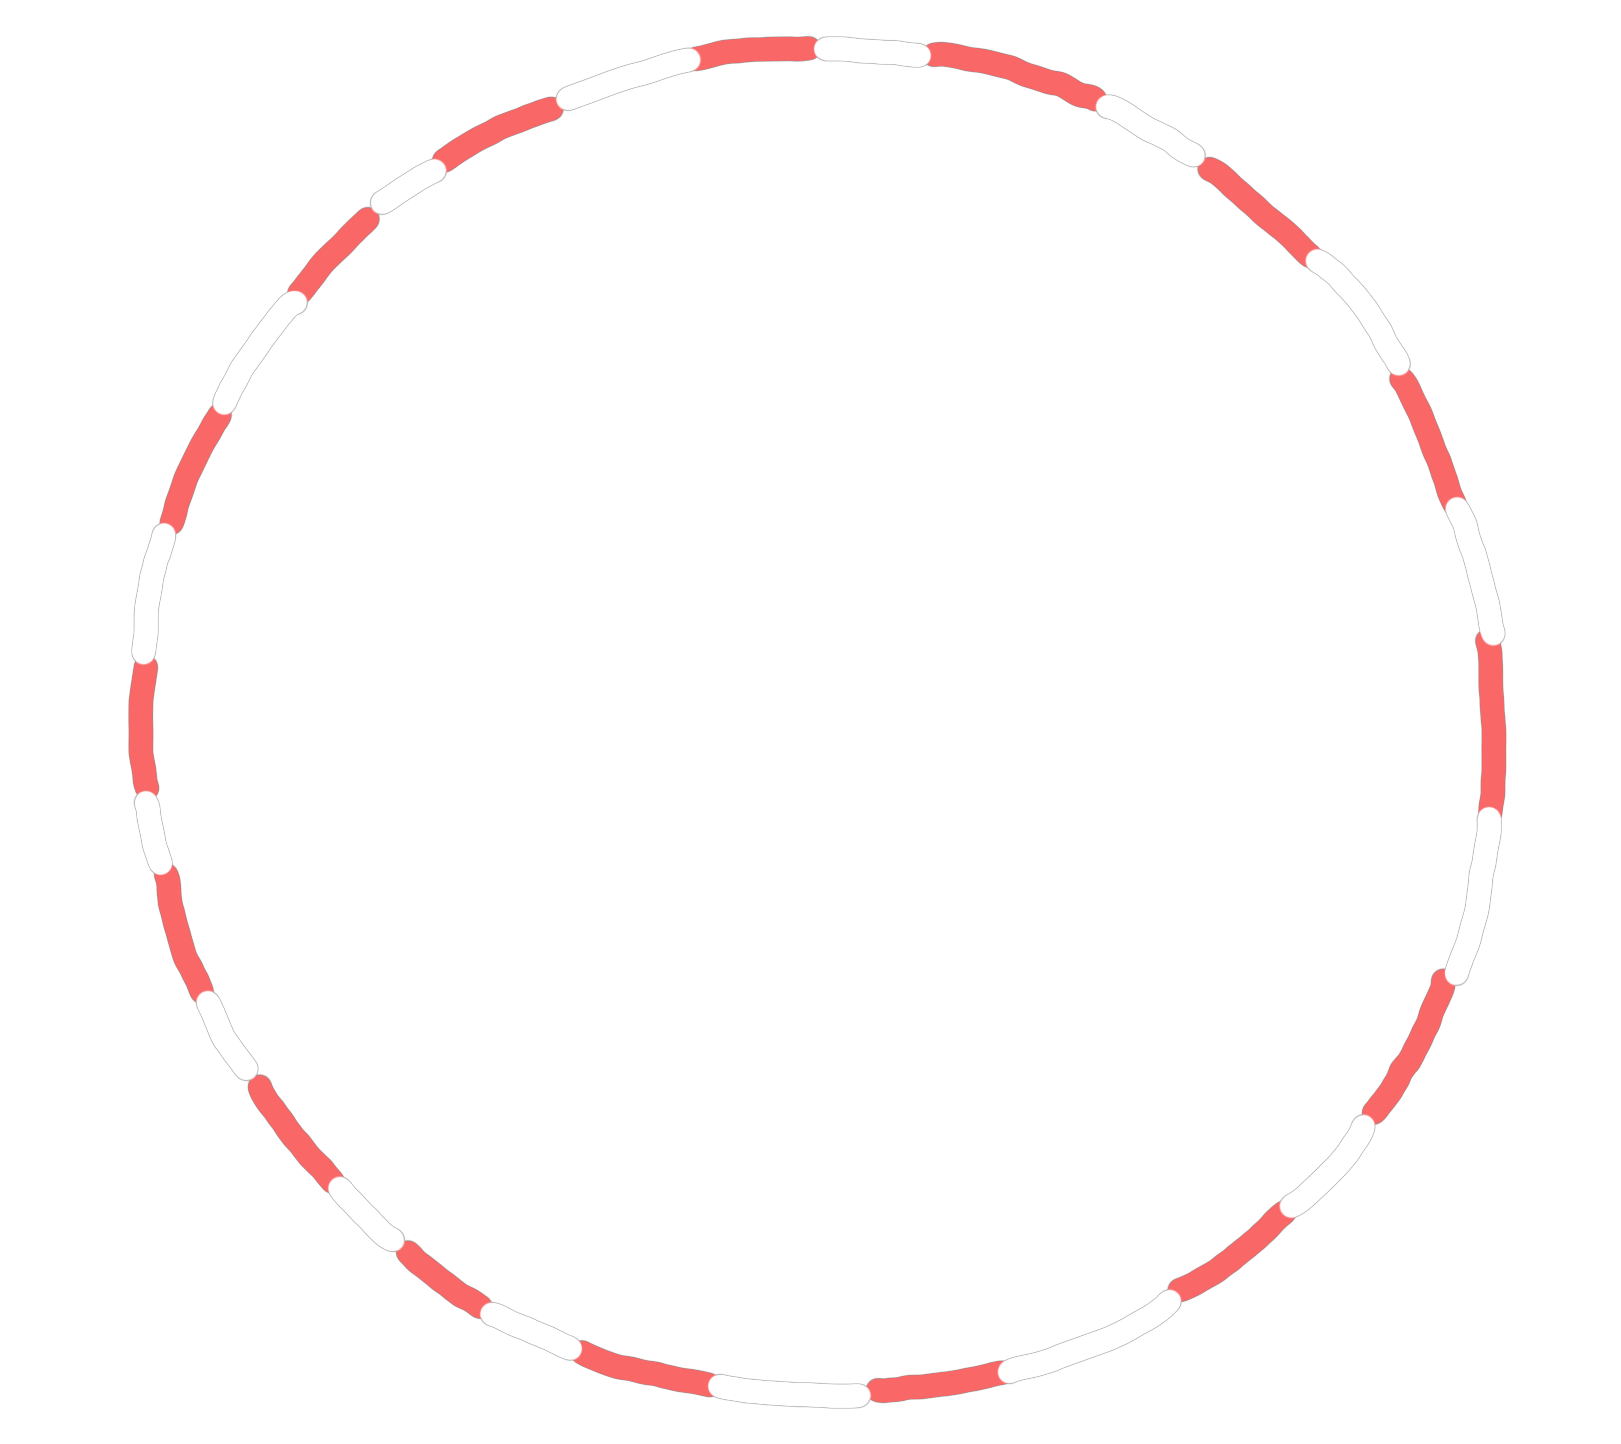
\includegraphics[width=1\linewidth]{bai6}
		\vspace*{-5pt}
	\end{figure}
	\textit{Lời giải.} Để chiến thắng được Mãng xà, Thạch Sanh phải chém đứt được một số chẵn cái đầu của nó. Số đầu mới của Mãng xà sẽ tăng thêm chỉ trong trường hợp nếu Thạch Sanh chém đứt một số cái đuôi nào của con  chằn tinh này. Do có tất cả $3$ cái đuôi, nên nếu chém đứt tất cả đuôi của Mãng xà, thì số đầu mới mọc ra không ít hơn  $2$ cái. Vì thế tổng số đầu mà Thạch Sanh cần phải chém để thắng không ít hơn $5$ cái. Do vậy, một số chẵn cái đầu cần chém đứt phải tối thiểu là $6$ cái. Đây là cách Thạch Sanh tiêu diệt Mãng xà với $6$ đầu: Đầu tiên, chàng sẽ lần lượt chặt đứt từng cái đuôi (với $3$ nhát gươm). Mãng xà giờ có $6$ đuôi mới và $3$ đầu. Sau đó chàng lần lượt sẽ chặt đứt từng cặp đuôi (với $3$ nhát gươm). Lúc này Mãng xà giờ có $6$ đầu và $0$ đuôi. Cuối cùng Thạch Sanh sẽ lần lượt chặt từng cặp $2$ cái đầu sau $3$ nhát chém. Tóm lại, với $9$ nhát gươm Thạch Sanh sẽ hạ được con chằn tinh.
\end{multicols}
\newpage
\begingroup
\thispagestyle{toancuabinone}
\blfootnote{$^1$\color{toancuabi}Canada.}
\AddToShipoutPicture*{\put(60,733){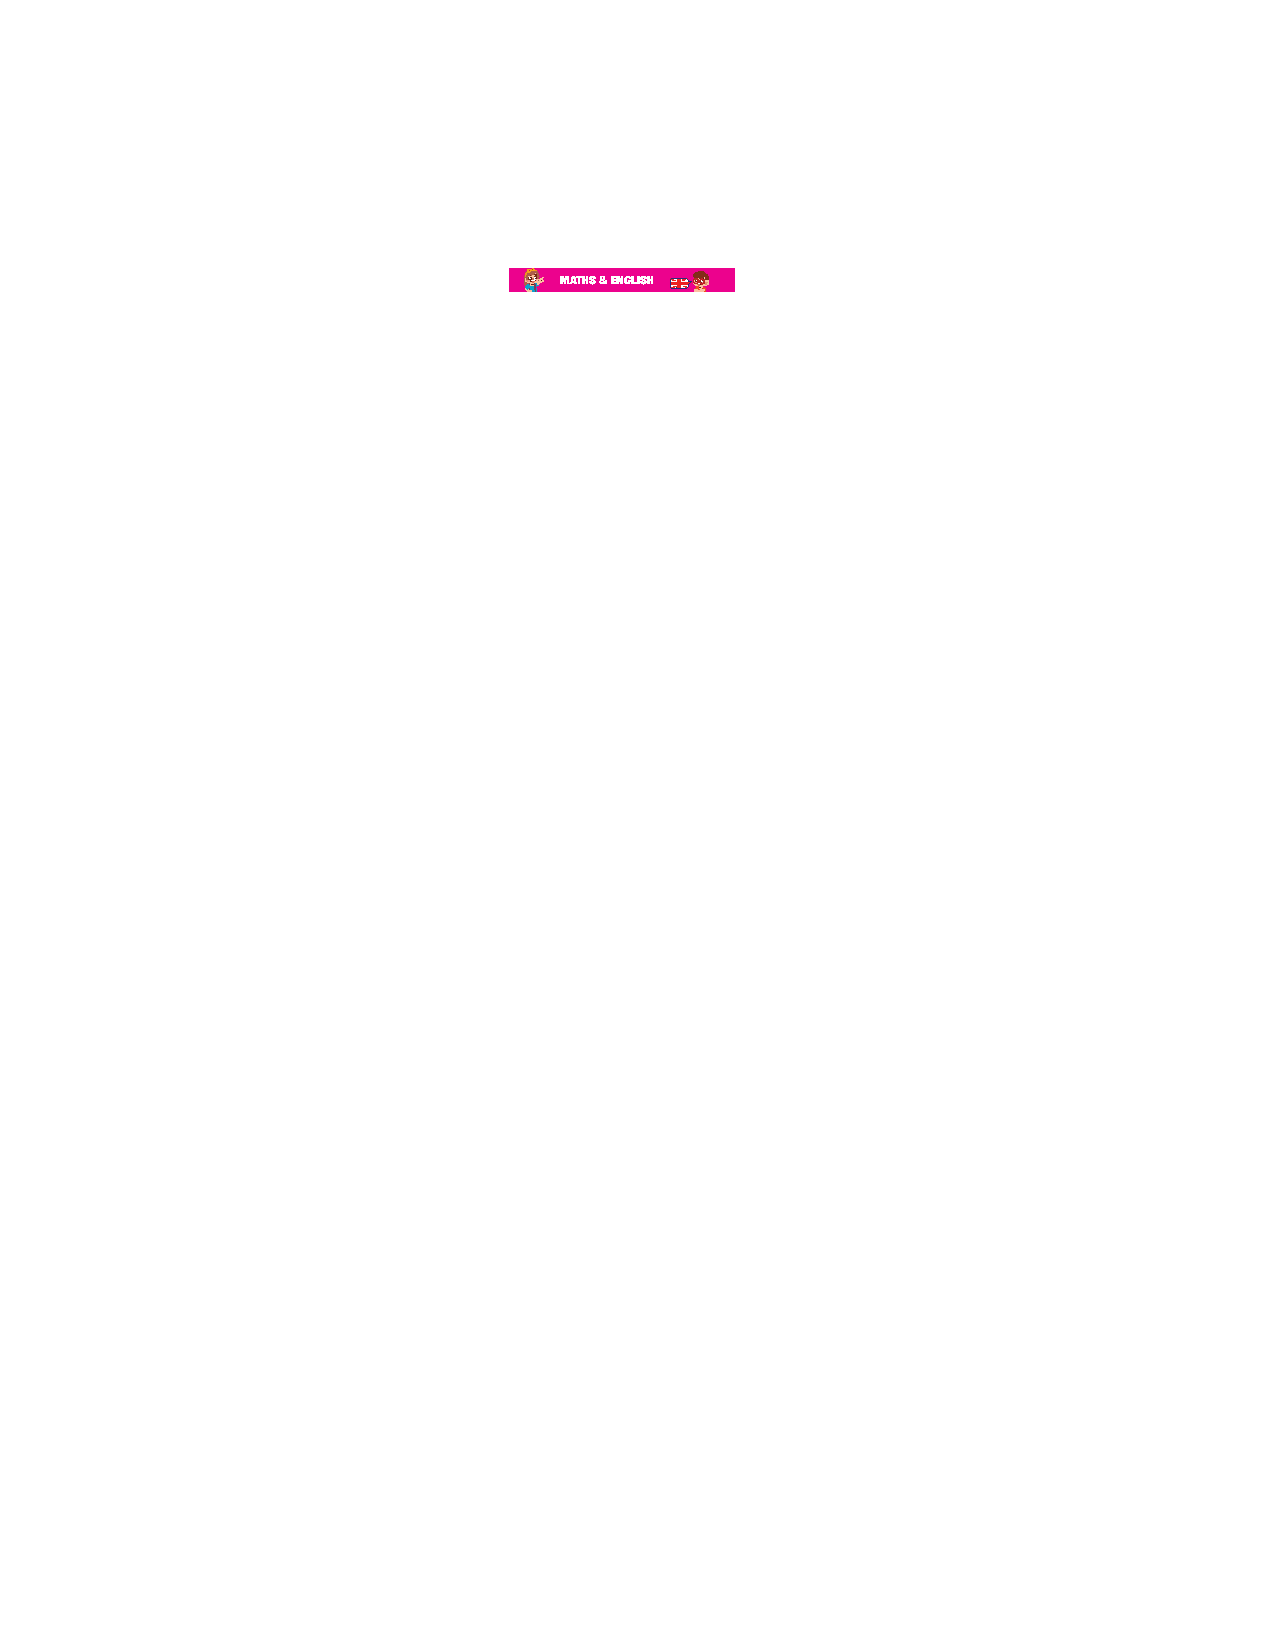
\includegraphics[width=17.2cm]{../mathc.pdf}}}
%\AddToShipoutPicture*{\put(-2,733){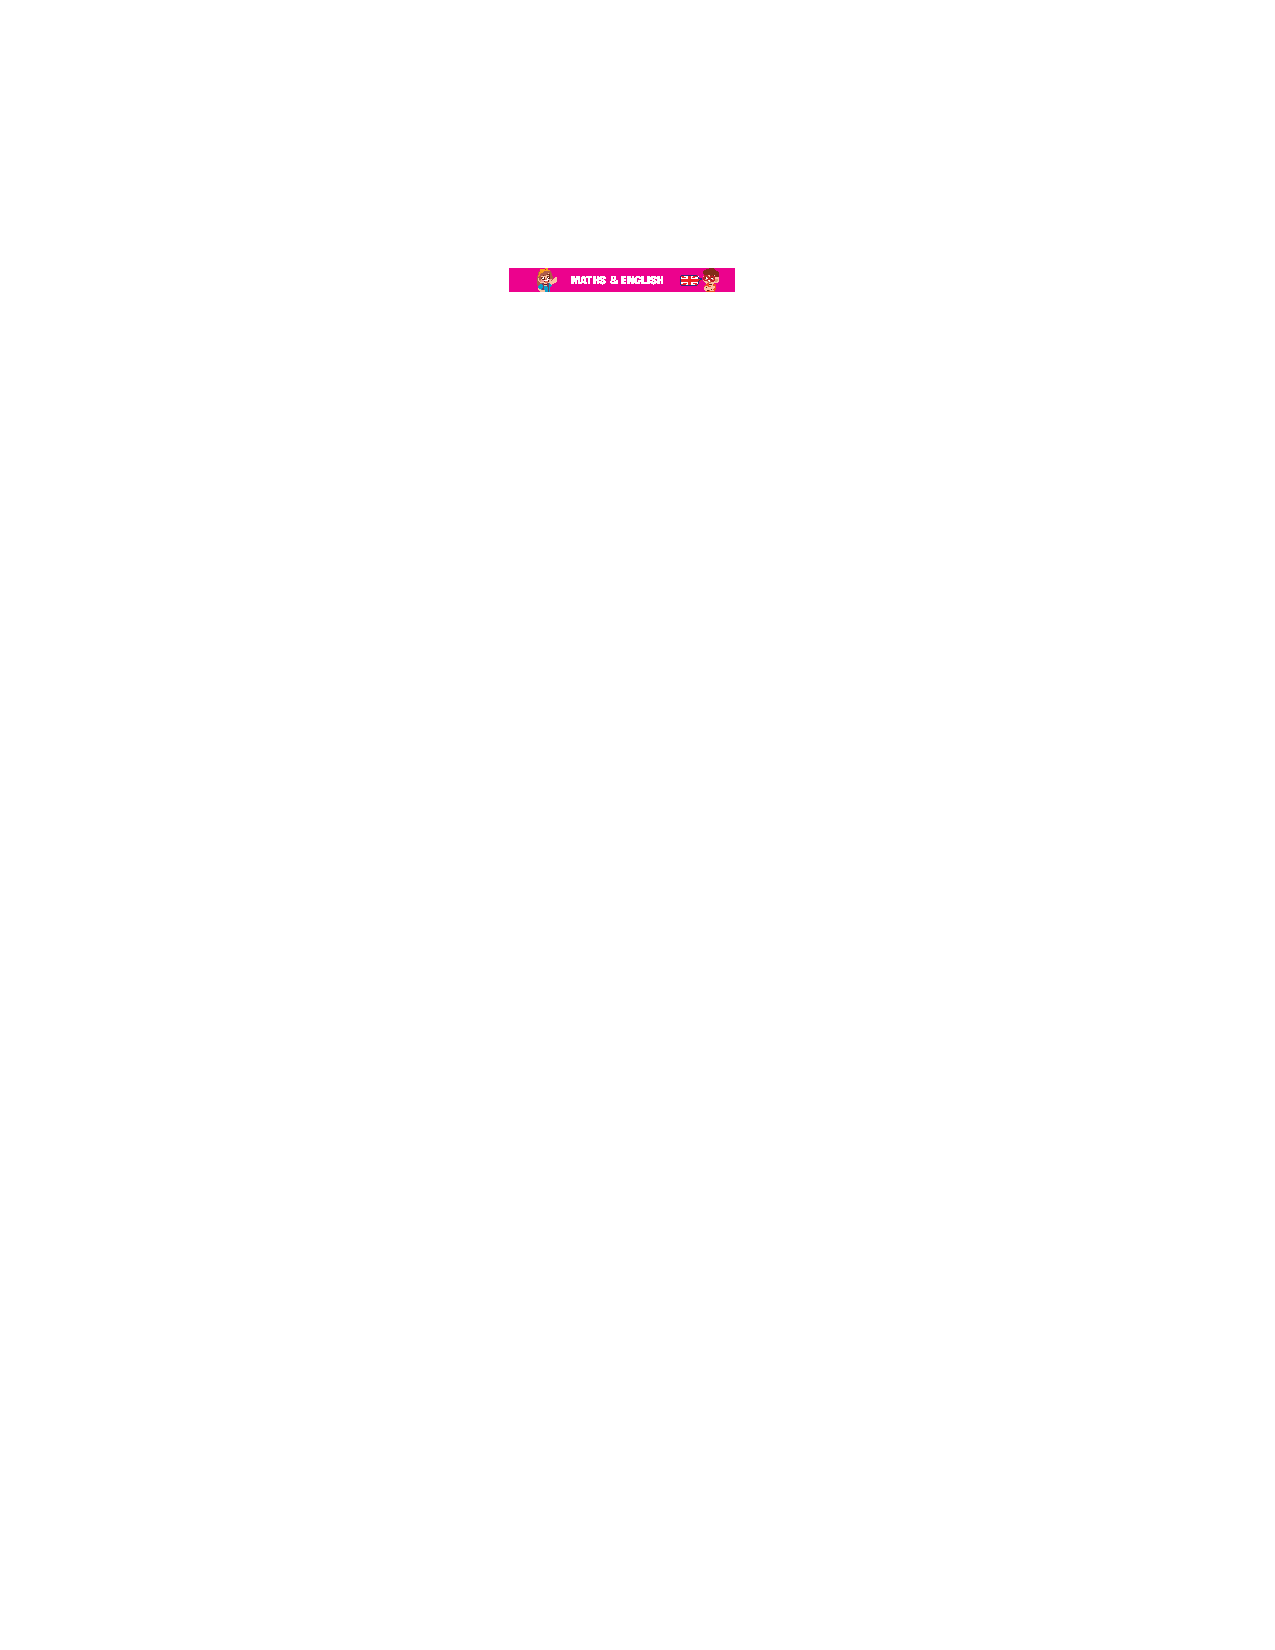
\includegraphics[width=17.2cm]{../mathl.pdf}}} 
\AddToShipoutPicture*{\put(88,675){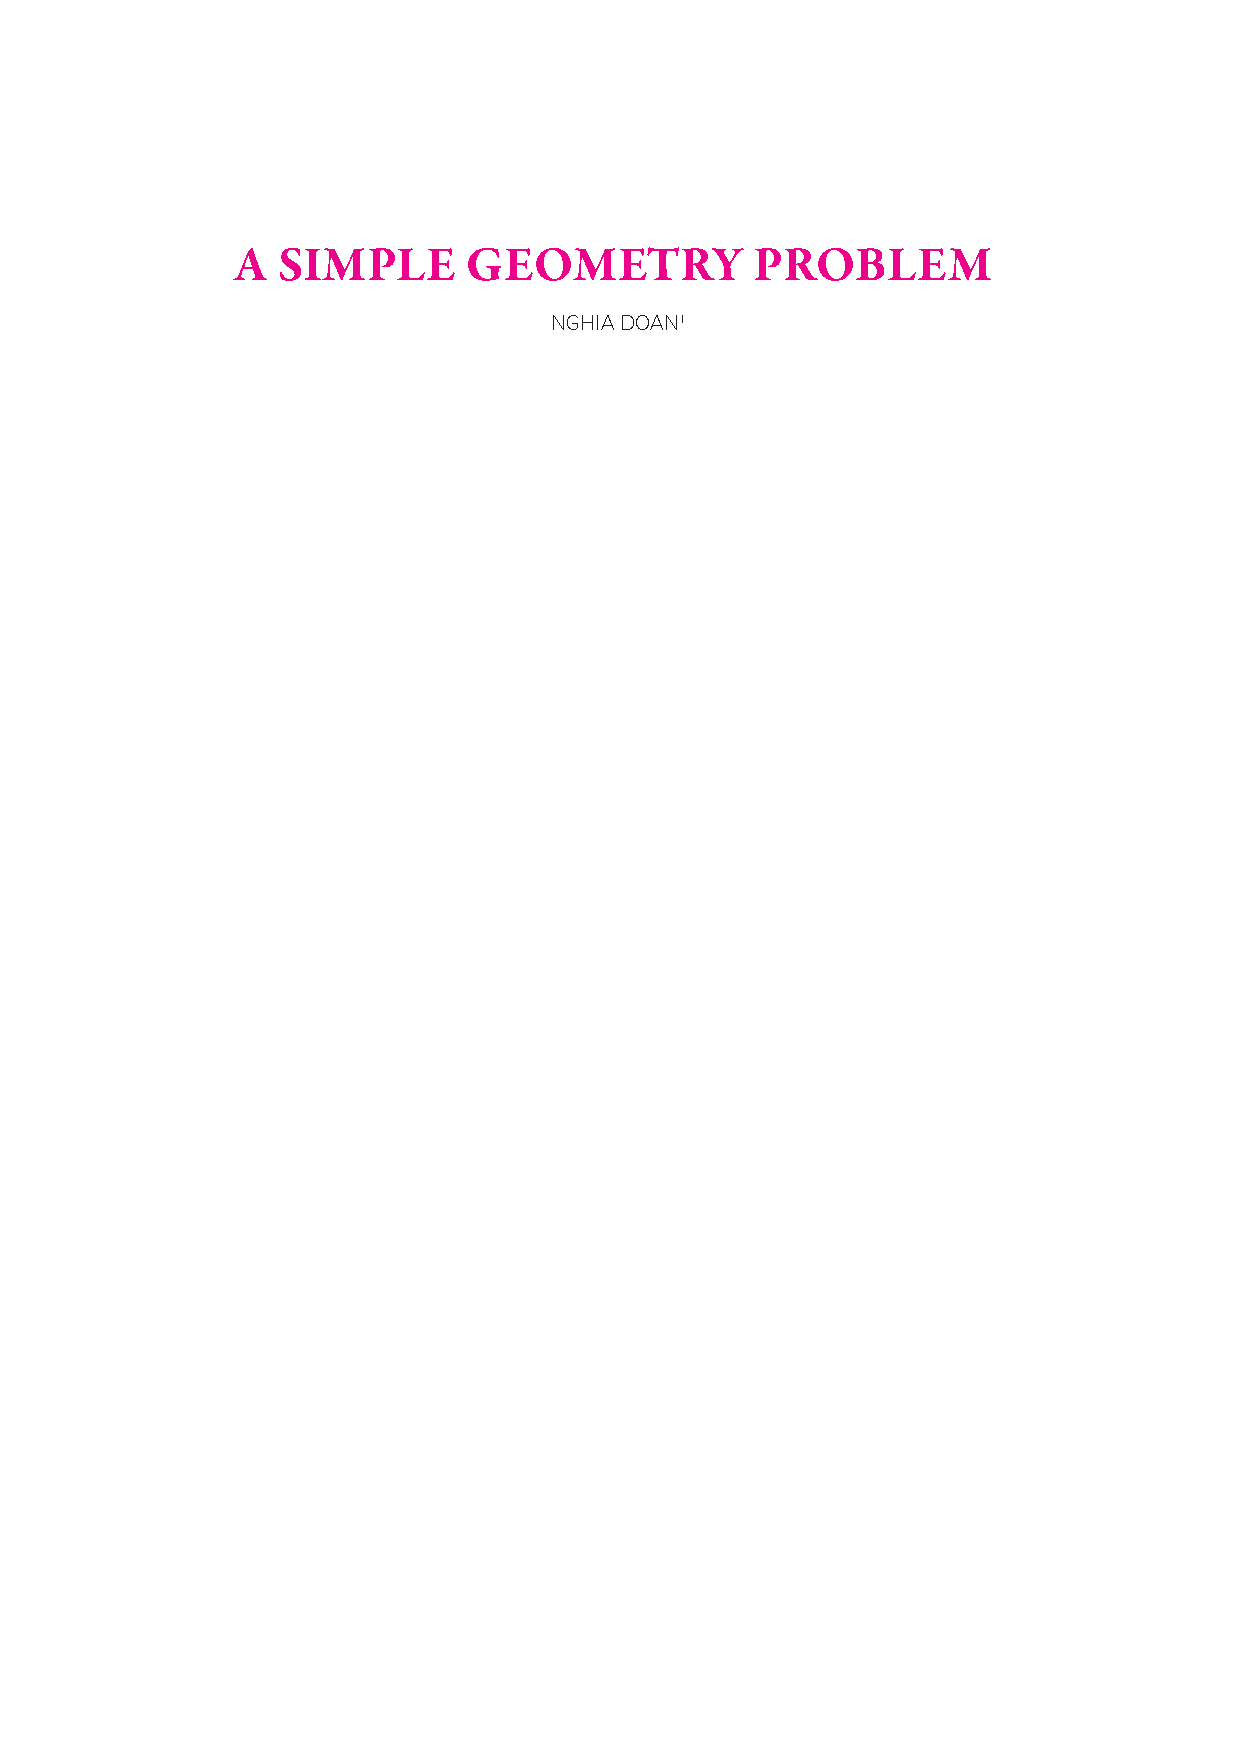
\includegraphics[scale=1]{../tieude3.pdf}}} 
\centering
\endgroup
\graphicspath{{../toancuabi/pic/}}
\vspace*{35pt}

\begin{multicols}{2}
	Usually approaching a problem from different angles help to see different nature of the problem,
	more importantly of what we learned, and how to apply them.
	In this article, we shows five different approaches, or solutions, to a simple geometry problem.
	\vskip 0.2cm
	\PIbox{\textbf{\color{toancuabi}Example}
	\vskip 0.1cm
	Let $ABCD$ be a square, $E$ is the midpoint of side $AD,$
	and $F$ is the foot of the altitude from $C$ to $BE.$
	Prove that $DF = DA.$}
	\begin{figure}[H]
		\vspace*{-5pt}
		\centering
		\captionsetup{labelformat= empty, justification=centering}
		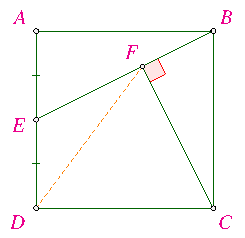
\includegraphics[width= 0.7\linewidth]{2022-2-ms-1-1.pdf}
		\vspace*{-15pt}
	\end{figure}
	\textit{First proof -- Using congruent triangles}.
	Extending $FE$ to intersect $CD$ at $G,$ see the diagram on the left. 
	Since $\angle AEB = \angle GED, AE = ED, \angle EAB = \angle EDA = 90^\circ,$
	by the angle-side-angle (ASA) rule, the triangles $ EAB$ and $EDG,$ are equal,
	thus the corresponding pair of sides are the same, or $DG=AB$. Therefore $DG=DC.$
	\begin{figure}[H]
		\vspace*{-5pt}
		\centering
		\captionsetup{labelformat= empty, justification=centering}
		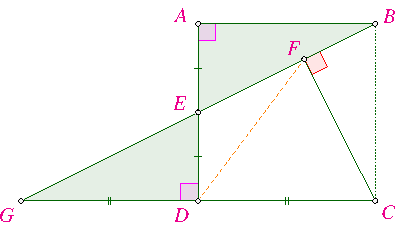
\includegraphics[width= 1\linewidth]{2022-2-ms-1-1-a.pdf}
		\vspace*{-15pt}
	\end{figure}
	\begin{figure}[H]
		\vspace*{-5pt}
		\centering
		\captionsetup{labelformat= empty, justification=centering}
		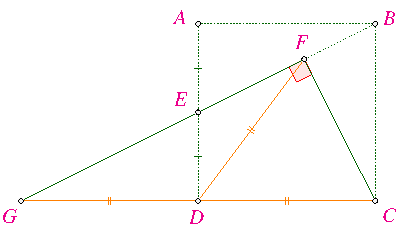
\includegraphics[width= 0.9\linewidth]{2022-2-ms-1-1-b.pdf}
		\vspace*{-10pt}
	\end{figure}	
	Now, it is a well--known fact that,
	\textit{the midpoint of the hypotenuse of a right triangle is at equidistance from all vertices.}
	Using this fact for $\triangle DGC$ in the diagram on the right in the figure above, $DG=DC,\ \angle{GFC} = 90^\circ,$ thus $DF=DG=DC.$
	\vskip 0.1cm
	\textit{Second proof -- Using median segment.}
	Let $G$ be the midpoint of $BC,$ and let $DG$ intersect $FC$ at $H.$
	By side--side--side (SSS) rule, the triangle $ EAB$ and $  GCD$ are equal,
	so $\angle ABE = \angle CDG$, implying $EB \parallel DG.$
	\begin{figure}[H]
		\vspace*{-15pt}
		\centering
		\captionsetup{labelformat= empty, justification=centering}
		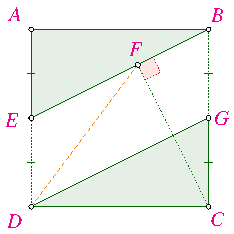
\includegraphics[width= 0.65\linewidth]{2022-2-ms-1-1-c.pdf}
		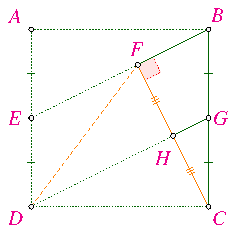
\includegraphics[width= 0.65\linewidth]{2022-2-ms-1-1-d.pdf}
		\vspace*{-5pt}
	\end{figure}	
	Furthermore, in $\triangle FBC,$ $GH \parallel BF,$ $G$ is midpoint of $BC,$
	so $H$ is midpoint of $FC.$
	Finally, in $\triangle DFC,$ $DH \perp FC,$ $H$ is midpoint of $FC,$
	thus by side--angle--side (SAS) rule, the triangles $ DHF$ and $DHC$ are equal, hence $DF = DC.$
	\begin{figure}[H]
		\vspace*{-10pt}
		\centering
		\captionsetup{labelformat= empty, justification=centering}
		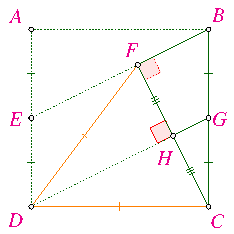
\includegraphics[width= 0.65\linewidth]{2022-2-ms-1-1-e.pdf}
		\vspace*{-15pt}
	\end{figure}		
	\textit{Third proof -- Using angles in circle}.
	The triangles $EDC$ and $ EFC$ are right at $D$ and $F$ respectively. It follows that the points $C, D, E$ and $F$ are on the circle centered at $G.$
	\begin{figure}[H]
		\vspace*{-15pt}
		\centering
		\captionsetup{labelformat= empty, justification=centering}
		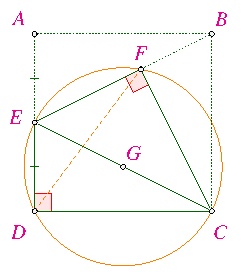
\includegraphics[width= 0.65\linewidth]{2022-2-ms-1-1-f.pdf}
		\captionsetup{labelformat= empty, justification=centering}
		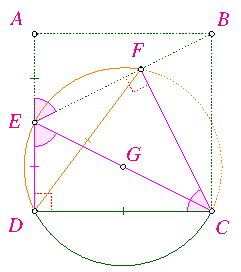
\includegraphics[width= 0.65\linewidth]{2022-2-ms-1-1-g.pdf}
		\vspace*{-5pt}
	\end{figure}	
	$\angle DEC = \angle AEB = 180^{\circ} - \angle DEF = \angle DCF.$ 
	$\angle DEC = \angle DFC$ (subtends arc $DC$).
	$\angle DCF = \angle DFC$, $\triangle DCF$ is isosceles, thus $DC = DF.$
	\vskip 0.1cm
	\textit{Fourth proof -- Using triangle trigonometry}.
	First, by Pythagorean theorem, $EB = \sqrt{AB^2 +AE^2} = \frac{a\sqrt{5}}{2}.$
	Then, let $\alpha = \angle DCF = \angle FBC = \angle AEB.$
	It is easy to see that $\cos{\alpha} = \frac{AE}{EB} = \frac{1}{\sqrt{5}},$
	and since $\triangle FCB \sim \triangle ABE$, $\frac{FC}{BC} = \sin{\alpha} = \frac{AB}{EB} = \frac{2}{\sqrt{5}},$
	so $FC = BC \sin{\alpha} = \frac{2a}{\sqrt{5}}.$
	\begin{figure}[H]
		\vspace*{-10pt}
		\centering
		\captionsetup{labelformat= empty, justification=centering}
		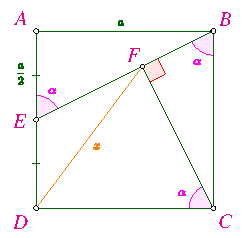
\includegraphics[width= 0.65\linewidth]{2022-2-ms-1-1-h.pdf}
		\vspace*{-15pt}
	\end{figure}	
	By the Law of Cosines,
	\begin{align*}
		DF &= \sqrt{DC^2 +  FC^2 - 2(DC)(FC)\cos{\alpha}}\\
		&= \sqrt{a^2 + \left(\frac{2a}{\sqrt{5}}\right)^2 - 2a \frac{2a}{\sqrt{5}} \frac{1}{\sqrt{5}}} = a.
	\end{align*}
	\textit{Fifth proof -- Using Ptolemy theorem}.
	Similar to the previous proof,
	let $DC = a \Rightarrow EB = EC = \frac{a\sqrt{5}}{2}.$ 
	$\frac{FC}{BC} = \frac{AB}{EB} \Rightarrow FC=\frac{2a}{\sqrt{5}}.$
	$\frac{FB}{BC} = \frac{AE}{EB} \Rightarrow FB=\frac{a}{\sqrt{5}}.$
	\begin{figure}[H]
		\vspace*{-15pt}
		\centering
		\captionsetup{labelformat= empty, justification=centering}
		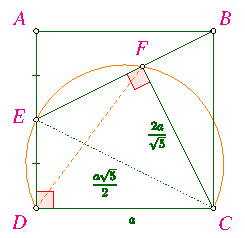
\includegraphics[width= 0.65\linewidth]{2022-2-ms-1-1-i.pdf}
		\vspace*{-15pt}
	\end{figure}	
	By Ptolemy theorem for the cyclic quadrilateral $CDEF,$
	$DF \cdot EC = ED \cdot FC + EF \cdot DC 
	= \frac{a}{2}\cdot \frac{2a}{\sqrt{5}} + \left(\frac{a\sqrt{5}}{2} - \frac{a}{\sqrt{5}} \right) \cdot a
	= \frac{a^2\sqrt{5}}{2} \Rightarrow DF = a.$
	\vskip 0.1cm
	Be open minded. Look for alternative approach. Try to use your own toolbox before looking for something else.
	Often you know more than you think you know.
\end{multicols} 
\begin{tBox}
	\centerline{\color{toancuabi}\textbf{New Words}}
	\vspace*{-10pt}
	\begin{multicols}{2}
		{\color{toancuabi}Geometry}: (dt) hình học
		\vskip 0.1cm
		{\color{toancuabi}Angle}: (dt) góc
		\vskip 0.1cm
		{\color{toancuabi}Triangle}: (dt) tam giác 
		\vskip 0.1cm
		{\color{toancuabi}Square}: (dt) hình vuông
		\vskip 0.1cm
		{\color{toancuabi}Quadrilateral}: (dt) tứ giác
		\vskip 0.1cm 
		{\color{toancuabi}Circle}: (dt) đường tròn  
		\vskip 0.1cm
		{\color{toancuabi}Midpoint}: (dt) trung điểm
		\vskip 0.1cm
		{\color{toancuabi}Median}: (dt) đường trung bình  
		\vskip 0.1cm
		{\color{toancuabi}Vertex}: (dt) đỉnh; (số nhiều: vertices).
		\vskip 0.1cm
		{\color{toancuabi}Altitude}: (dt) đường cao
		\vskip 0.1cm
		{\color{toancuabi}Congruent}: (tt) bằng nhau
		\vskip 0.1cm
		{\color{toancuabi}congruent triangles}: tam giác bằng nhau 
		\vskip 0.1cm
		{\color{toancuabi}Side}: (dt)  cạnh
		\vskip 0.1cm
		{\color{toancuabi}Hypotenuse}: (dt) cạnh huyền 
		\vskip 0.1cm
		{\color{toancuabi}Right}: (tt) vuông
		\vskip 0.1cm
		{\color{toancuabi}right angle}: góc vuông
		\vskip 0.1cm 
		{\color{toancuabi}Isoceleses}: (tt) cân
		\vskip 0.1cm
		{\color{toancuabi}isosceles triangle}: (dt) tam giác cân 
		\vskip 0.1cm
		{\color{toancuabi}Arc}: (dt) cung
	\end{multicols}
\end{tBox}
\vspace*{-10pt}
{\color{toancuabi}\rule{1\linewidth}{0.1pt}}
\vskip 0.2cm
{\centerline{\textbf{\LARGE\color{toancuabi}LỜI GIẢI, ĐÁP ÁN}}}
\begin{multicols}{2}
	Tiếp theo ta đánh số các thổ dân có màu xanh ngồi tiếp theo Toto theo chiều kim đồng hồ là $1, 2, 3,\ldots, 25$. 
	\vskip 0.1cm
	Ta nhận thấy mỗi một thổ dân luôn nói đúng tổng số tuổi của hai người ngồi cạnh mình. Ta sẽ lấy tổng các số tuổi được các thổ dân màu xanh ở vị trí số $1, 3, 5,\ldots, 23, 25$ nói ra. Đó chính là tổng số tuổi của tất cả các thổ dân màu  đỏ, cộng thêm tuổi của Toto. Sau đó ta lại lấy tổng các số tuổi được các thổ dân màu xanh ở vị trí số $2, 4, ,\ldots, 22, 24$ nói ra. Đây lại chính là tổng số tuổi của tất cả các thổ dân màu  đỏ, trừ đi tuổi của Toto. Lấy tổng đầu tiên trừ đi tổng thứ hai rồi chia đôi, ta nhận được ngay tuổi của anh Toto. Như vậy có thể biết tuổi của bất kỳ ai trong số $50$ thổ dân ăn mặc rất đẹp kia.
	\vskip 0.1cm
	Vậy em đã biết cách Xuân Phong xác định được ai là người đến từ tộc Tutu hay đến từ tộc Titi rồi chứ nào. Chắc hẳn Xuân Phong và Lê Kính đã có một kỳ nghỉ tuyệt vời bên cạnh những người thổ dân vui tính thật đặc biệt này.
	\vskip 0.1cm
	\textbf{\color{toancuabi}Góc cờ}
	\vskip 0.1cm
	\textbf{\color{toancuabi}$\pmb{1}$.b$\pmb{8}$/H+ Vxb$\pmb{8}$ $\pmb{2}$.Vb$\pmb{6}$ Ta$\pmb{2}$ $\pmb{3}$.Xc$\pmb{2}$ Tb$\pmb{3}$ $\pmb{4}$.Xb$\pmb{2}$!}
	\begin{center}
		\newgame
		\fenboard{1k6/8/1K6/8/8/1b6/1R6/8 b Q - 0 1}
		\scalebox{0.85}\showboard
	\end{center}
	\textbf{\color{toancuabi}$\pmb{4}$...Te$\pmb{6}$} [$4$...Tf$7$ $5$.Xf$2$ Te$6$ $6$.Xf$8$+ Tc$8$ $7$.Xd$8$; $4$...Ta$4$ $5$.Va$5$+; $4$...Td$5$ $5$.Xd$2$ Tb$7$ $6$.Xd$8$+ Tc$8$ $7$.Xf$8$]
	\vskip 0.1cm
	\textbf{\color{toancuabi}$\pmb{5}$.Xe$\pmb{2}$ Td$\pmb{7}$ $\pmb{6}$.Xh$\pmb{2}$ Vc$\pmb{8}$ $\pmb{7}$.Xh$\pmb{8}$+ Te$\pmb{8}$ $\pmb{8}$.Xxe$\pmb{8}$+}
\end{multicols}